\section{Histograms on the First Run~\label{sec:first_run}} 
This section exhibits histograms on the first run of 
INC with its task length increasing from 1 second to 4096 seconds. 
The detailed description of the base data is from Table~\ref{tab:exp_notes1}.

%\section{Experiment Notes}
\paragraph{Experiment Notes:}
Table~\ref{tab:exp_notes1} provides a short description of our experimental runs, 
on which the following histograms are based.

%% done
\begin{table}[h]
\begin{center}
\begin{tabular}{|p{2cm}|p{3cm}|p{3cm}|p{4cm}|p{3cm}|} \hline
Machine & Task Length (sec) & Description & Experiment Period & Relevant \linebreak Histograms\\ \hline
{\tt sodb9} &  INC1$\sim$INC64 & 1000 samples, each & 2017-03-02 $\sim$ 2017-03-04 & Figs.~\ref{fig:s9_r1_et_hist1},~\ref{fig:s9_r1_et_hist2},~\ref{fig:s9_r1_pt_hist1}, and~\ref{fig:s9_r1_pt_hist2}\\ \hline
{\tt sodb9} &  INC128$\sim$INC1024 & 300 samples, each & 2017-03-04 $\sim$ 2017-03-11 & 
Figs.~\ref{fig:s9_r1_et_hist3} and~\ref{fig:s9_r1_pt_hist3}\\ \hline
{\tt sodb10} & INC2048 & 300 samples & 2017-03-02 $\sim$ 2017-03-09 & Figs.~\ref{fig:inc2048_r1_et_hist_v5} and~\ref{fig:inc2048_r1_hist_v5}\\ \hline
{\tt sodb12} & INC4096 & 300 samples & 2017-02-13 $\sim$ 2017-02-27 & Figs.~\ref{fig:inc4096_r1_et_hist_v5} and~\ref{fig:inc4096_r1_hist_v5}\\ \hline
\end{tabular}
\end{center}
\vspace{-.2in}
\caption{Notes on experiment runs used for histograms\label{tab:exp_notes1}}
\end{table}

\pagebreak

\subsection{ET}

\begin{figure}[hp!]
	\centering
	\subfigure[ET frequency on INC1]{
		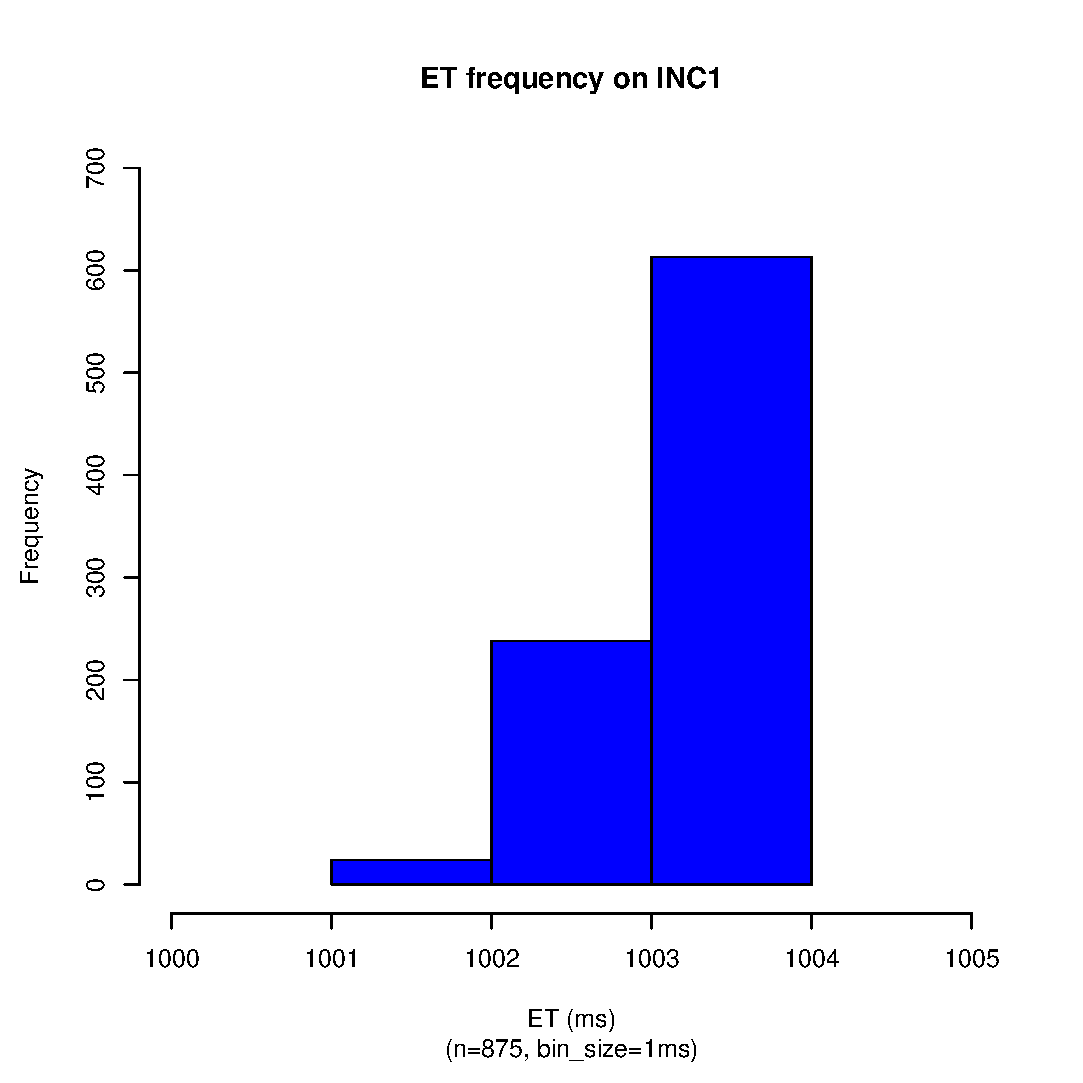
\includegraphics[scale=0.43]{repet_data1/1_sec_et_hist_v5.eps}
		\label{fig:inc1_r1_et_hist_v5}
	}
	\subfigure[ET frequency on INC2]{
		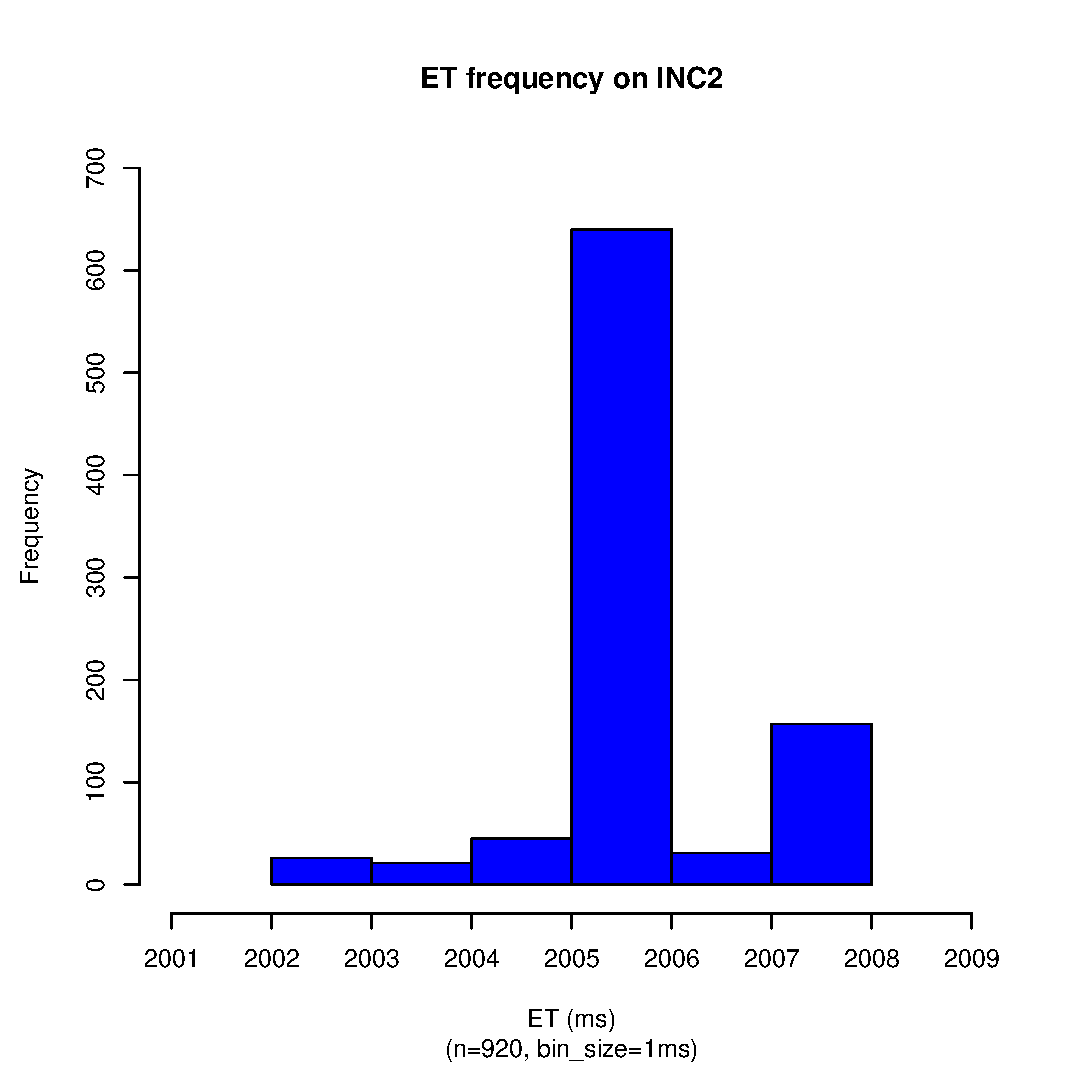
\includegraphics[scale=0.43]{repet_data1/2_sec_et_hist_v5.eps}
		\label{fig:inc2_r1_et_hist_v5}
	}
	\subfigure[ET frequency on INC4]{
		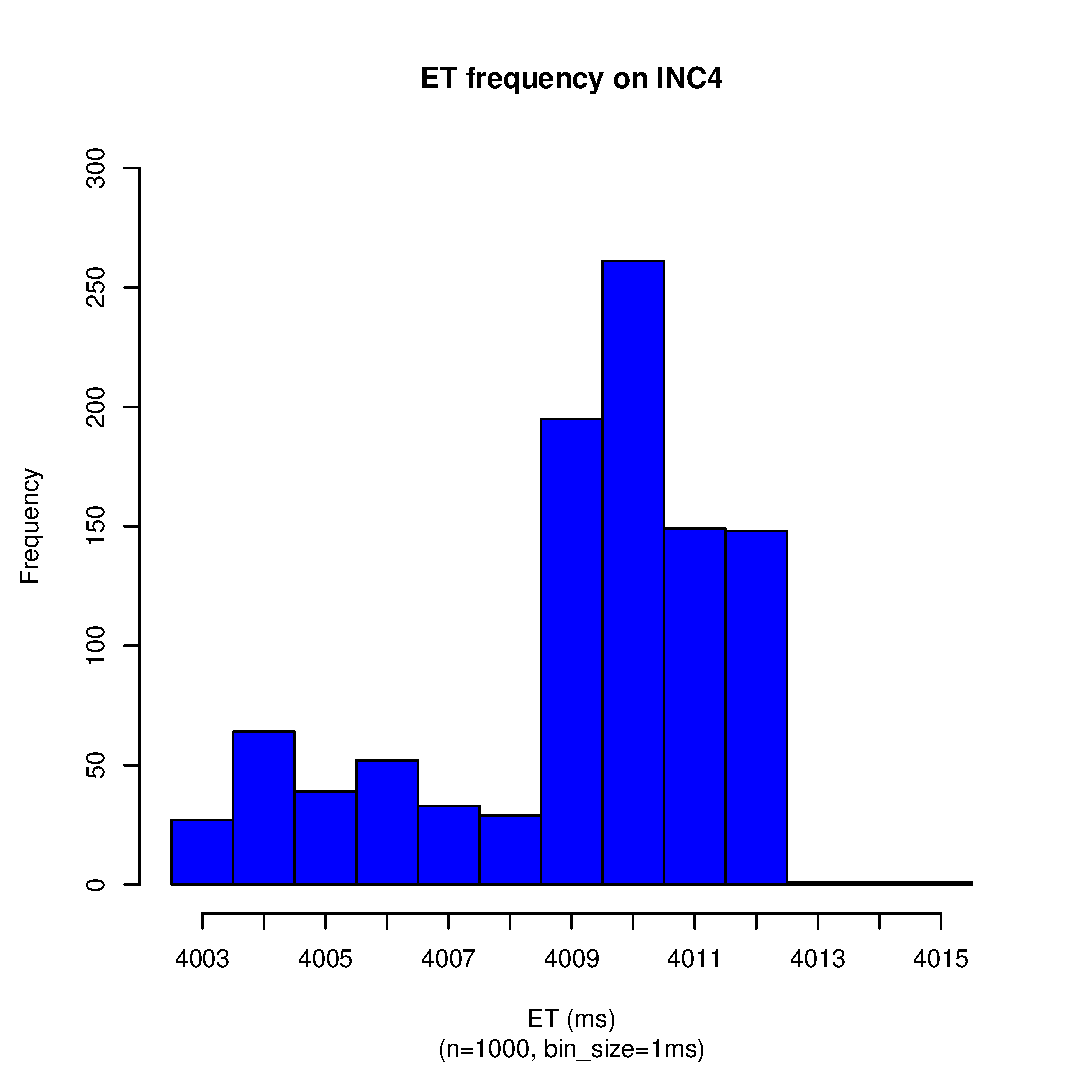
\includegraphics[scale=0.43]{repet_data1/4_sec_et_hist_v5.eps}
		\label{fig:inc4_r1_et_hist_v5}
	}
	\subfigure[ET frequency on INC8]{
		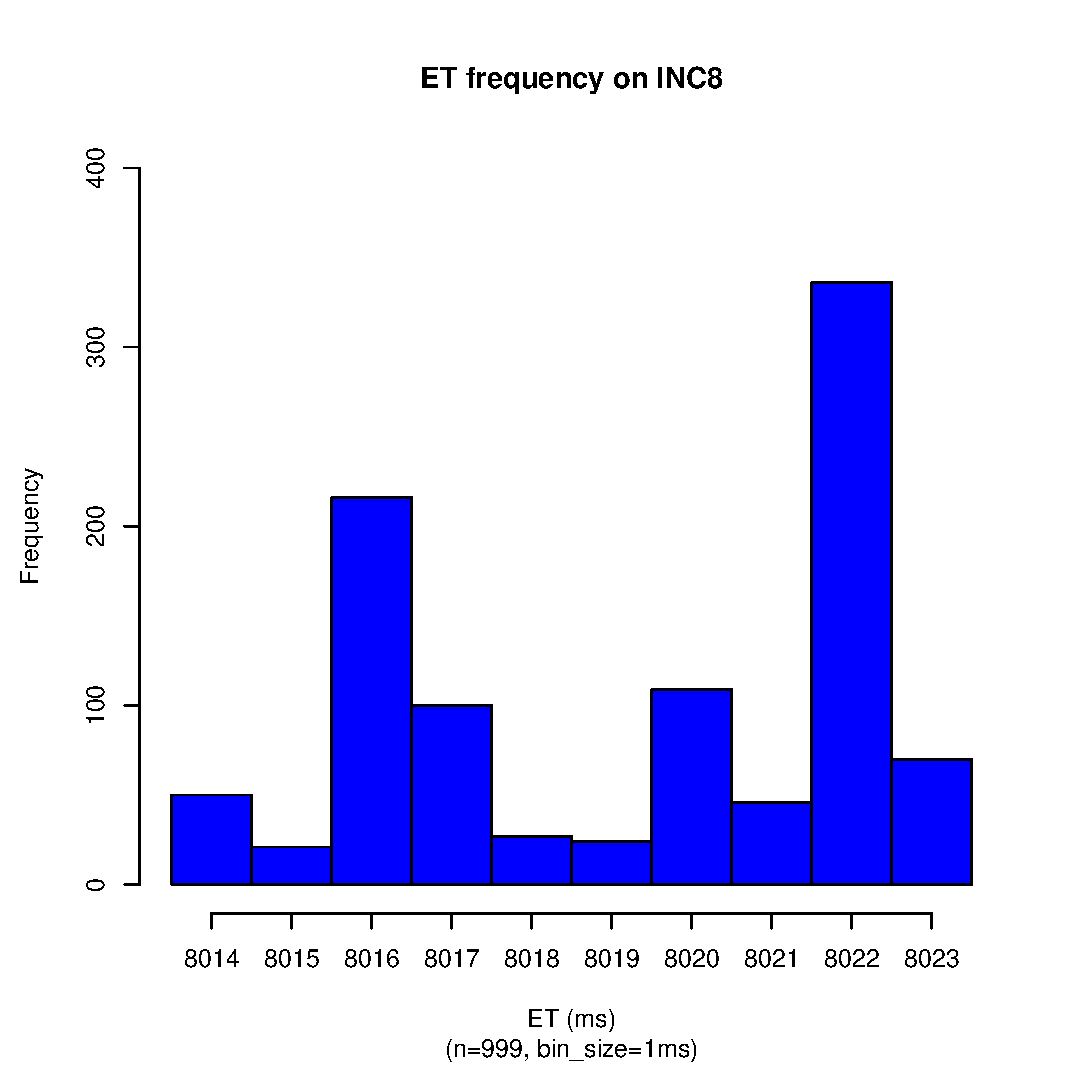
\includegraphics[scale=0.43]{repet_data1/8_sec_et_hist_v5.eps}
		\label{fig:inc8_r1_et_hist_v5}
	}
	\caption{ET Histograms of INC1 ... INC8~\label{fig:s9_r1_et_hist1}}
\end{figure}

\begin{figure}[hp!]
	\centering
	\subfigure[ET frequency on INC16]{
		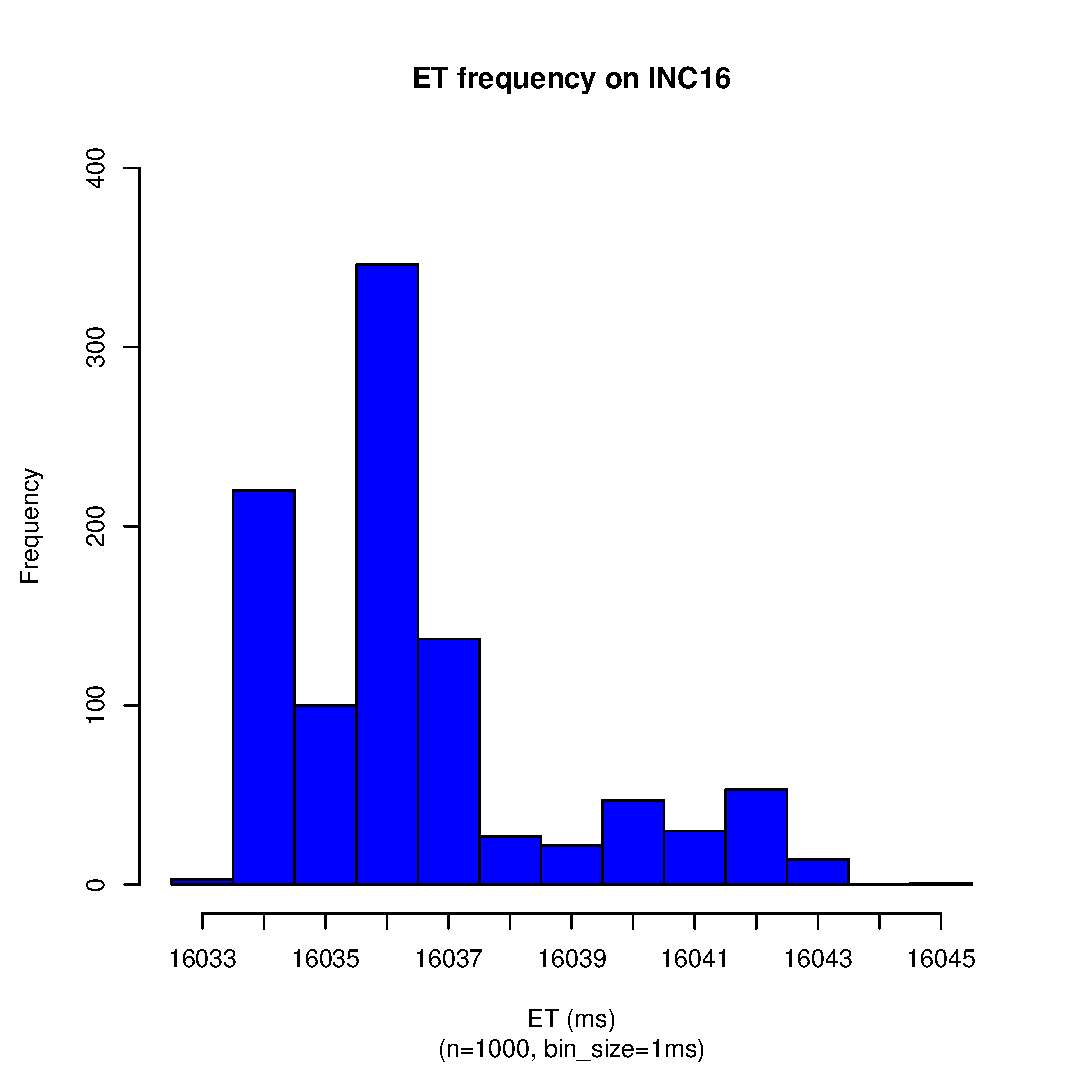
\includegraphics[scale=0.43]{repet_data1/16_sec_et_hist_v5.eps}
		\label{fig:inc16_r1_et_hist_v5}
	}
	\subfigure[ET frequency on INC32]{
		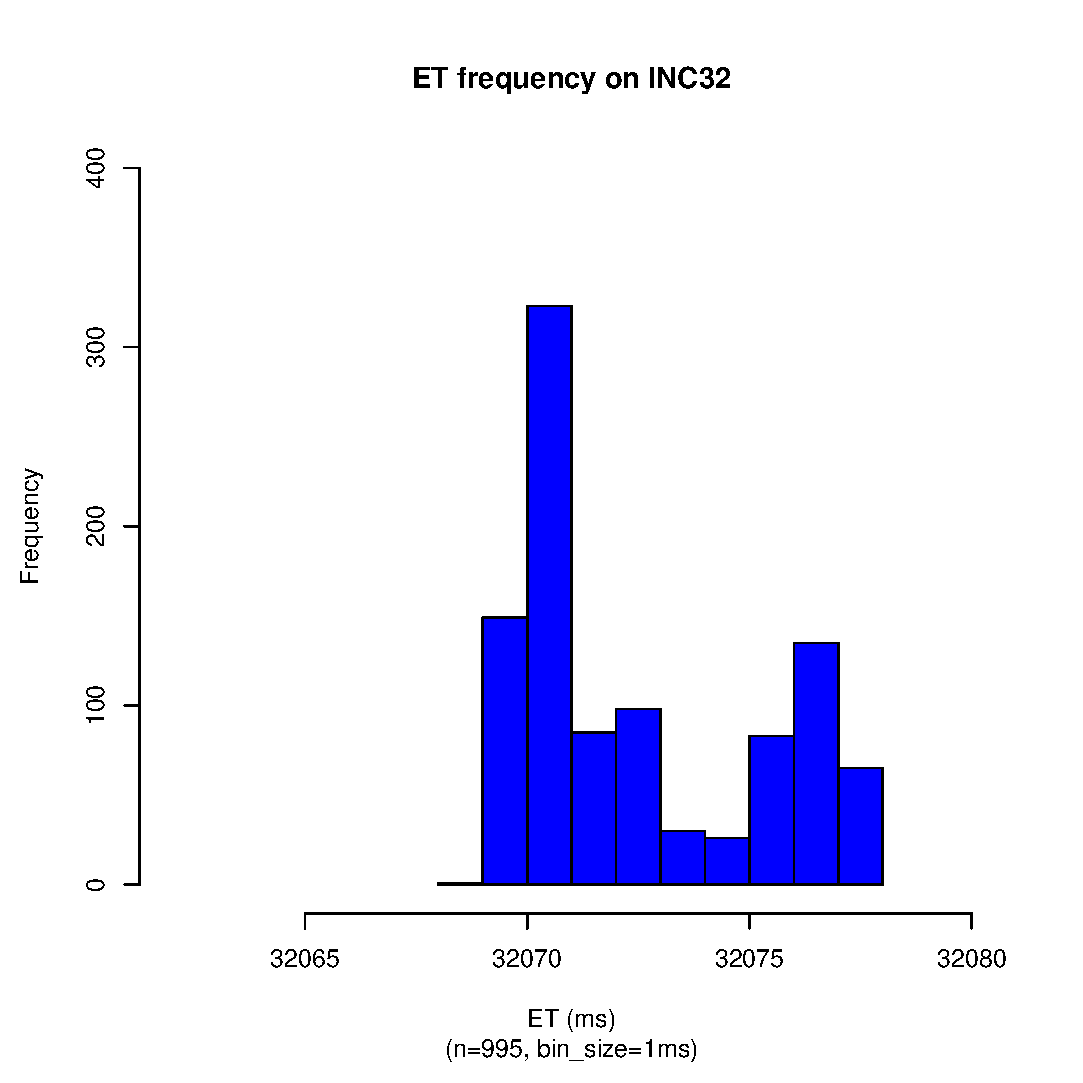
\includegraphics[scale=0.43]{repet_data1/32_sec_et_hist_v5.eps}
		\label{fig:inc32_r1_et_hist_v5}
	}
	\subfigure[ET frequency on INC64]{
		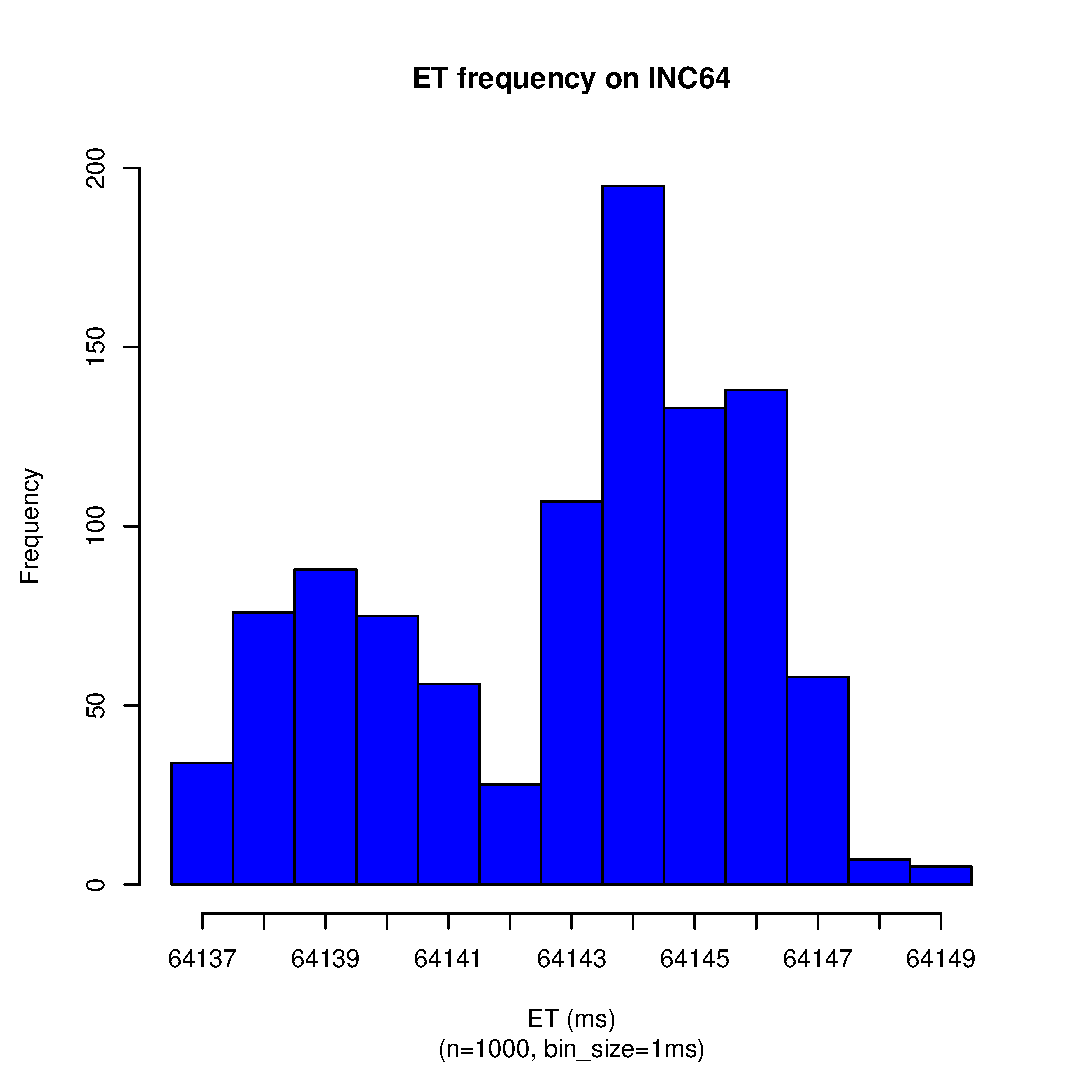
\includegraphics[scale=0.43]{repet_data1/64_sec_et_hist_v5.eps}
		\label{fig:inc64_r1_et_hist_v5}
	}
	\caption{ET Histograms of INC16 ... INC64~\label{fig:s9_r1_et_hist2}}
\end{figure}

\begin{figure}[hp!]
	\centering
	\subfigure[ET frequency on INC128]{
		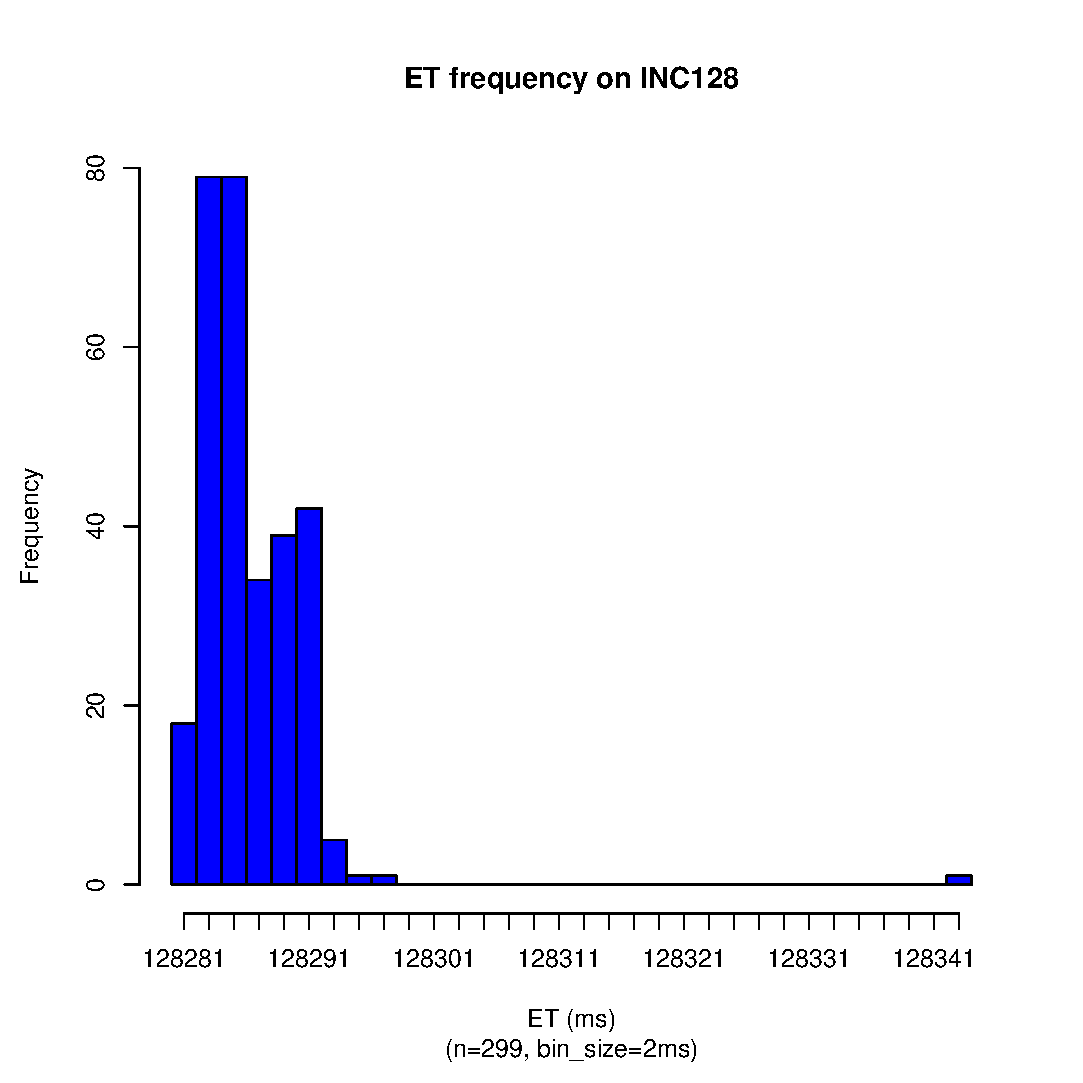
\includegraphics[scale=0.43]{repet_data1/128_sec_et_hist_v5.eps}
		\label{fig:inc128_r1_et_hist_v5}
	}
	\subfigure[ET frequency on INC256]{
		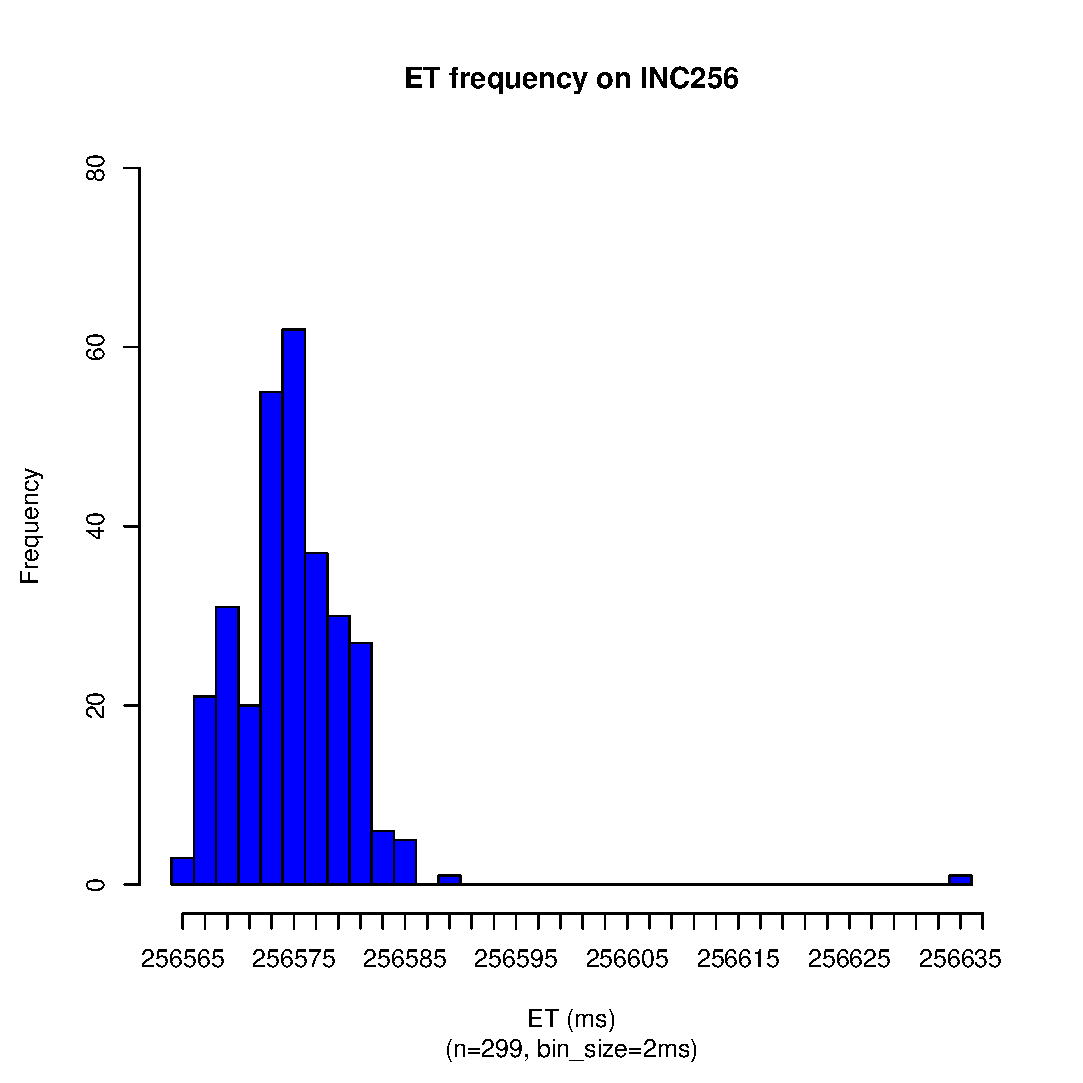
\includegraphics[scale=0.43]{repet_data1/256_sec_et_hist_v5.eps}
		\label{fig:inc256_r1_et_hist_v5}
	}
	\subfigure[ET frequency on INC512]{
		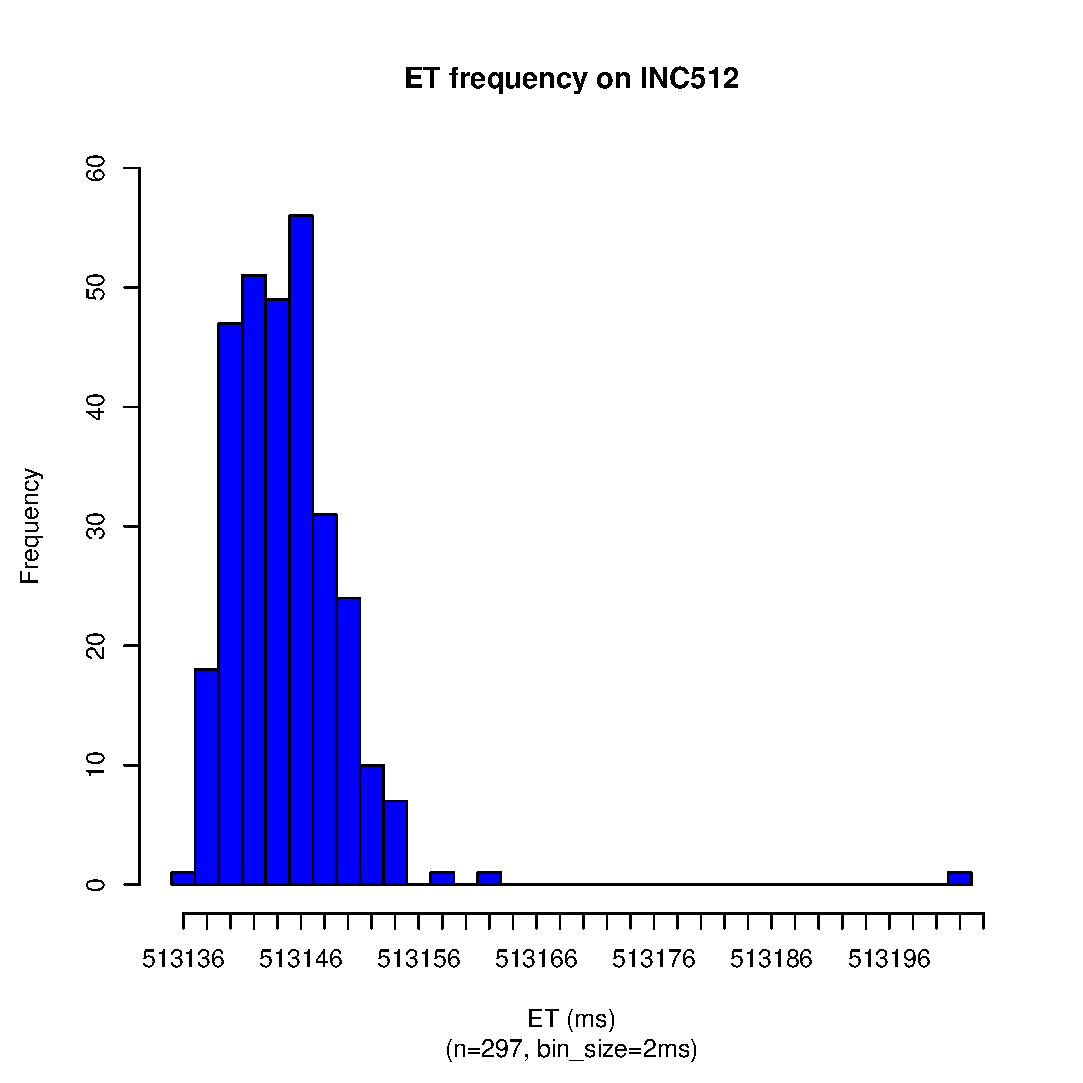
\includegraphics[scale=0.43]{repet_data1/512_sec_et_hist_v5.eps}
		\label{fig:inc512_r1_et_hist_v5}
	}
	\subfigure[ET frequency on INC1024]{
		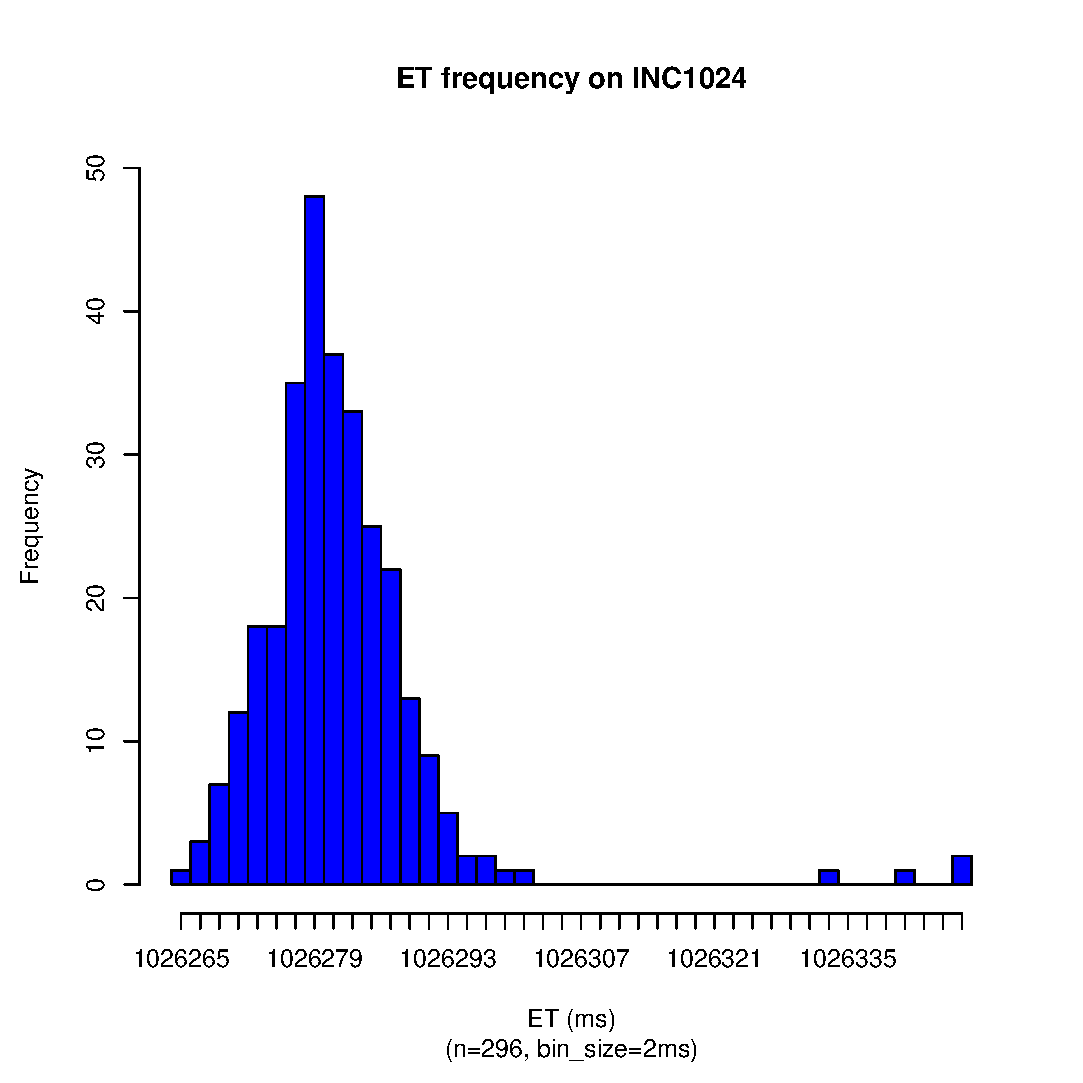
\includegraphics[scale=0.43]{repet_data1/1024_sec_et_hist_v5.eps}
		\label{fig:inc1024_r1_et_hist_v5}
	}
	\caption{ET Histograms of INC128 ... INC1024~\label{fig:s9_r1_et_hist3}}
\end{figure}

\pagebreak

\begin{figure}[t]
	\centering
	\subfigure[ET frequency on INC2048]{
		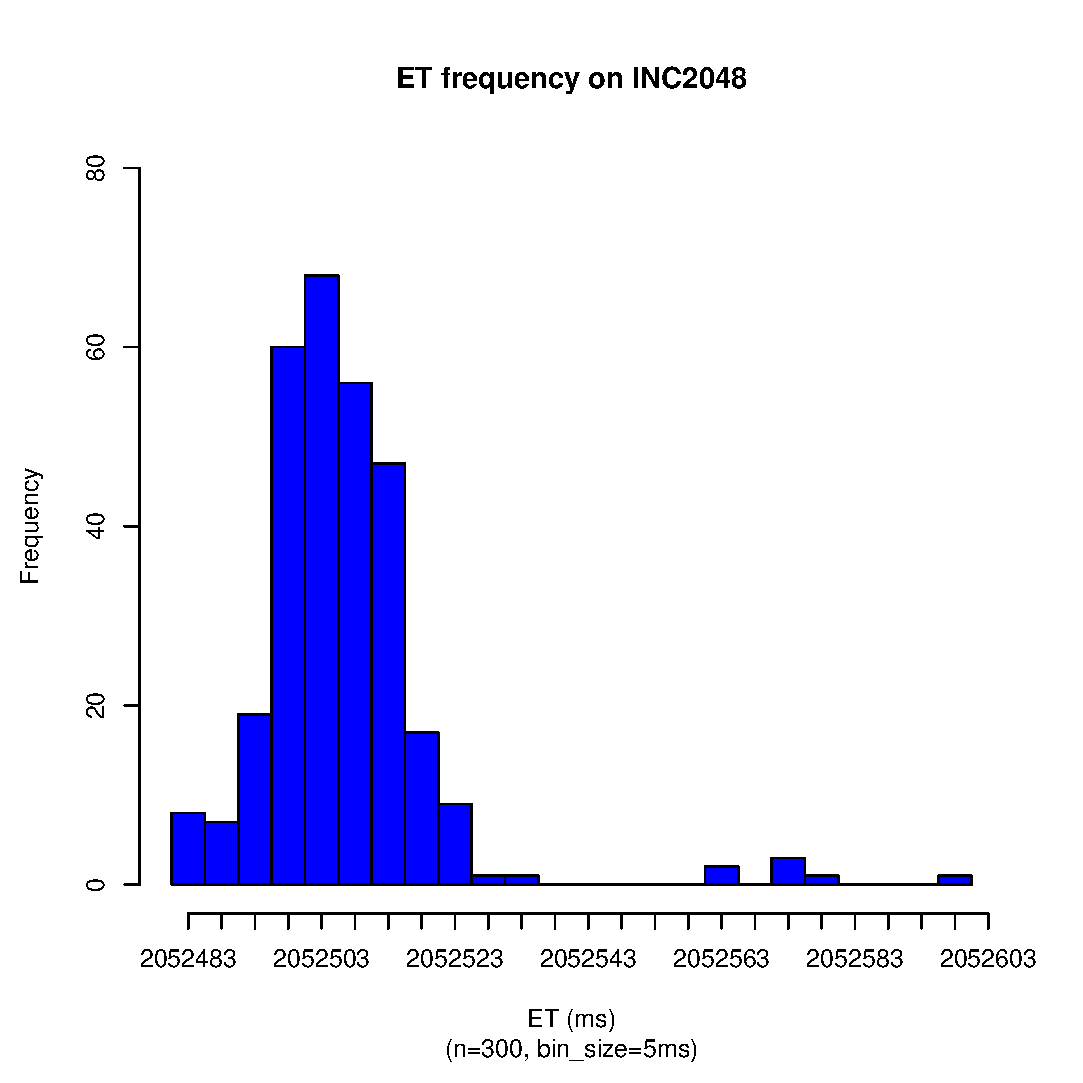
\includegraphics[scale=0.43]{repet_data1/2048_sec_et_hist_v5.eps}
		\label{fig:inc2048_r1_et_hist_v5}
	}
	\subfigure[ET frequency on INC4096]{
		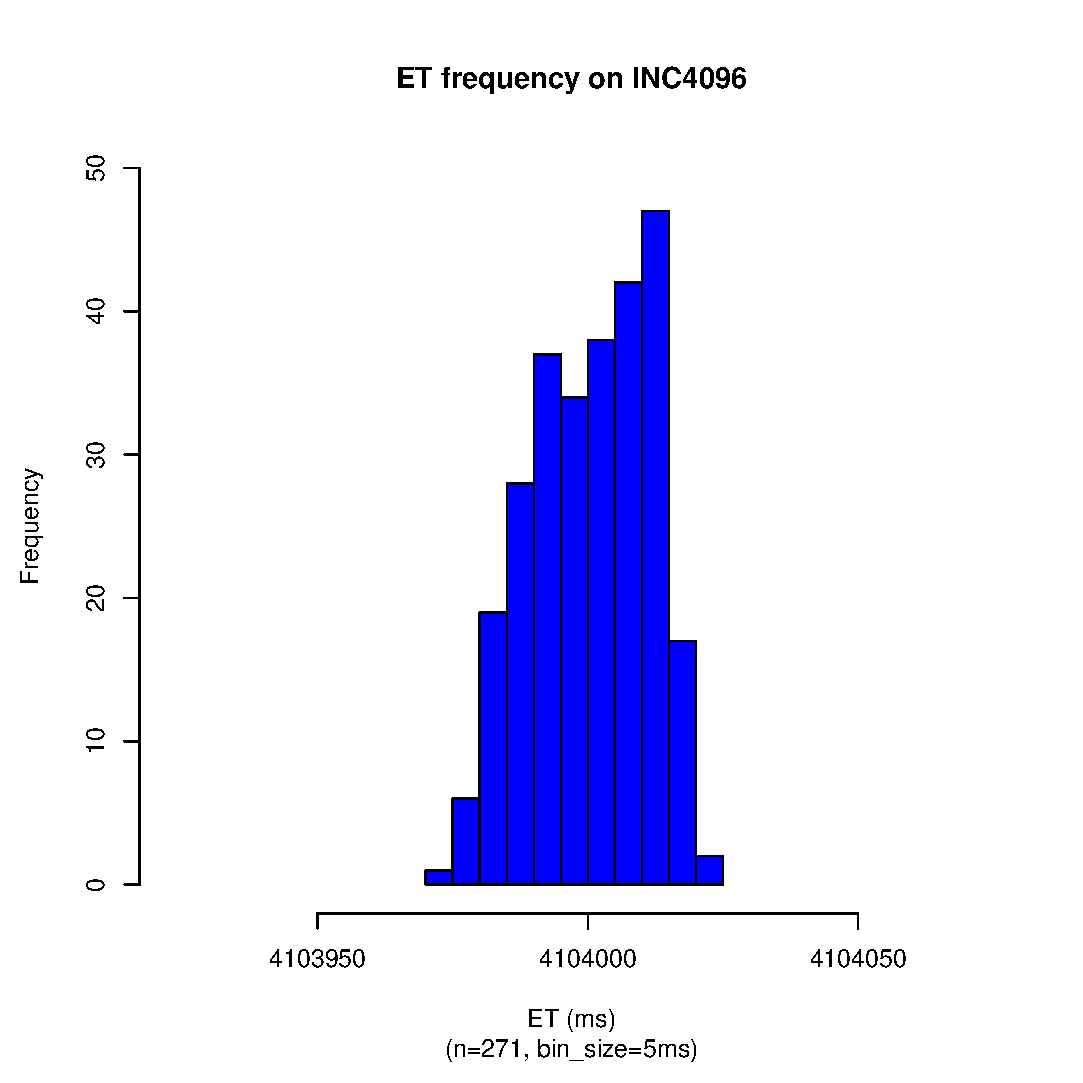
\includegraphics[scale=0.43]{repet_data1/4096_sec_et_hist_v5.eps}
		\label{fig:inc4096_r1_et_hist_v5}
	}
	\caption{ET Histograms of INC2048 and INC4096~\label{fig:s9_r1_et_hist4}}
\end{figure}

\vspace\fill
\clearpage

\subsection{PT}

\begin{figure}[hp!]
	\centering
	\subfigure[PT frequency on INC1]{
		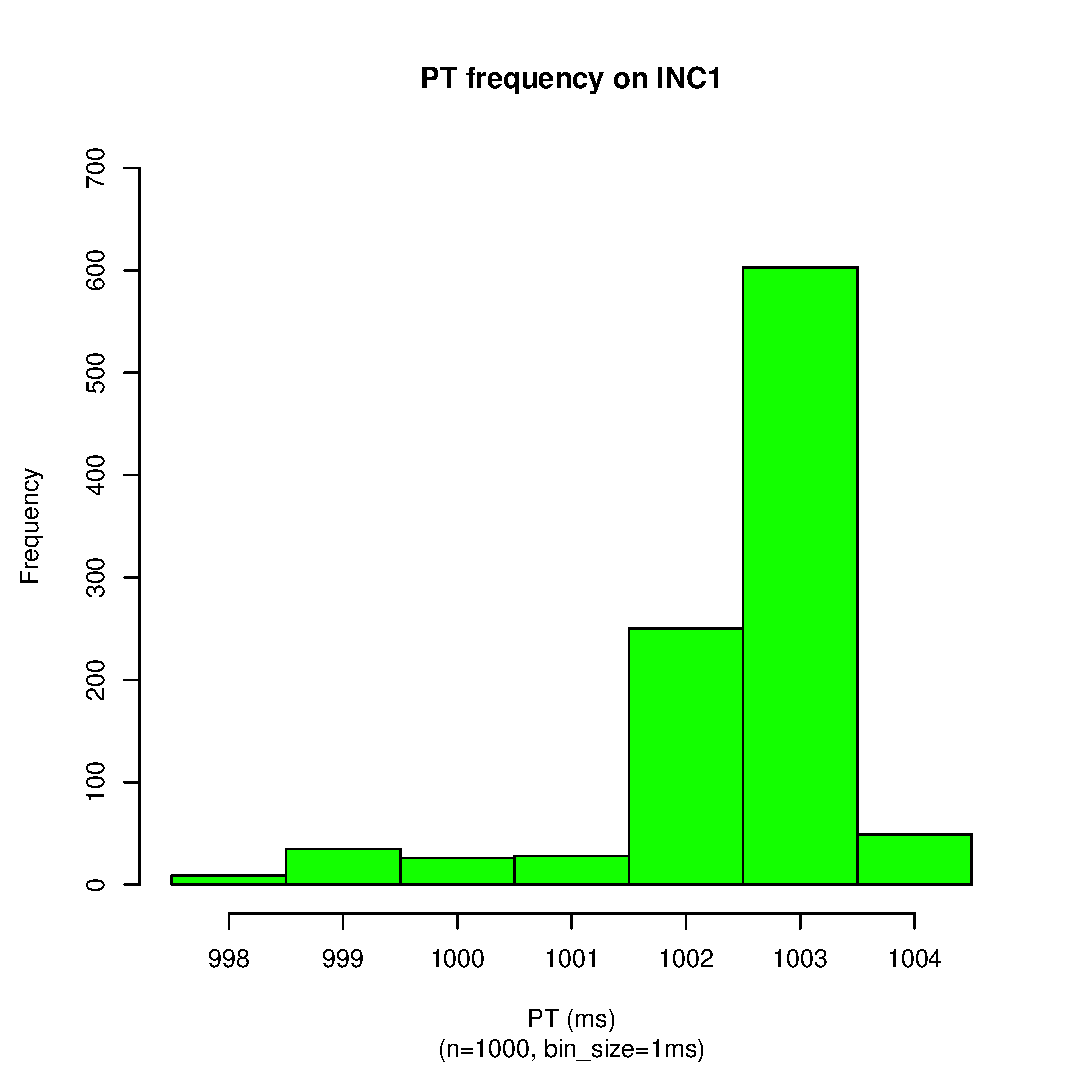
\includegraphics[scale=0.43]{repet_data1/1_sec_pt_hist_v5.eps}
		\label{fig:inc1_r1_hist_v5}
	}
	\subfigure[PT frequency on INC2]{
		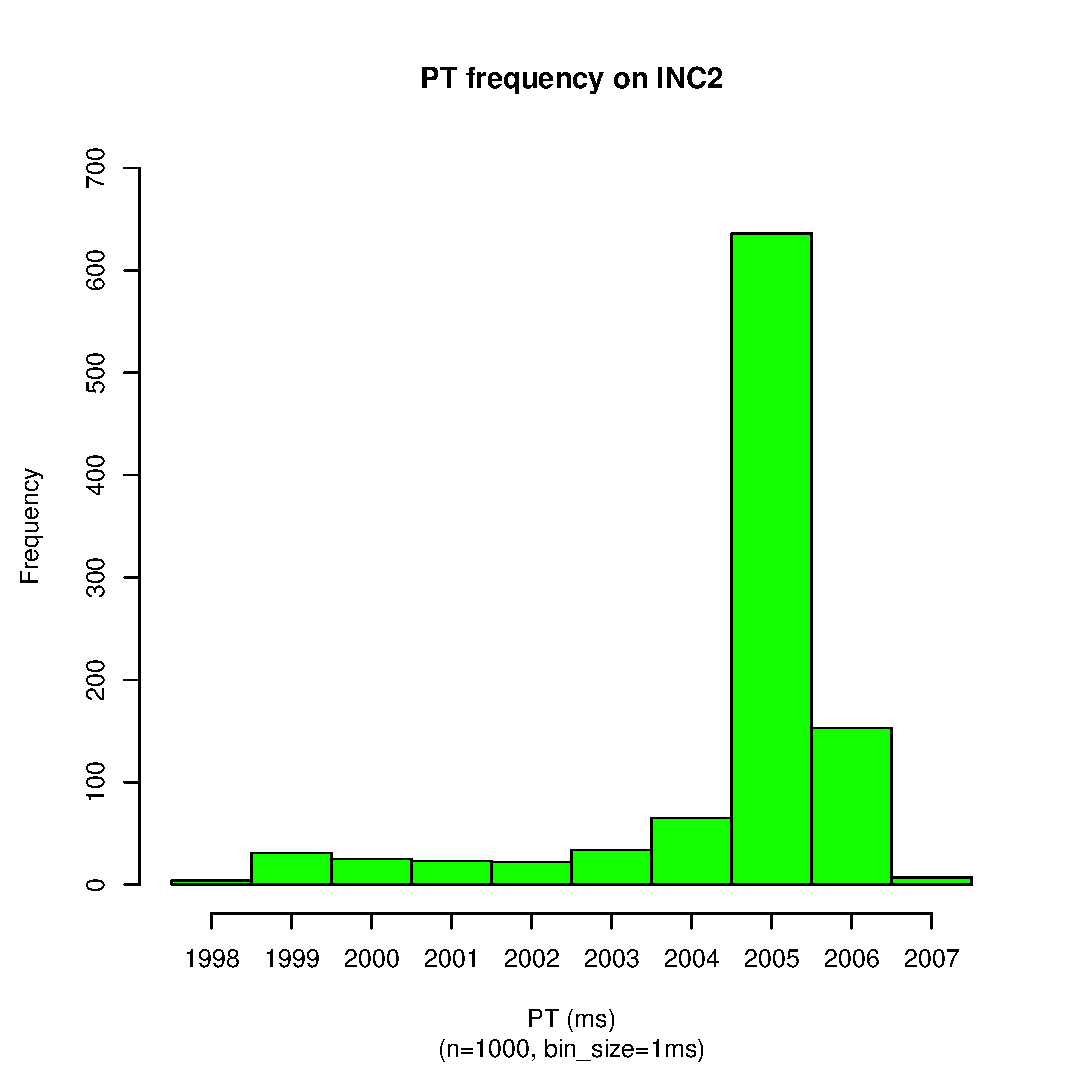
\includegraphics[scale=0.43]{repet_data1/2_sec_pt_hist_v5.eps}
		\label{fig:inc2_r1_hist_v5}
	}
	\subfigure[PT frequency on INC4]{
		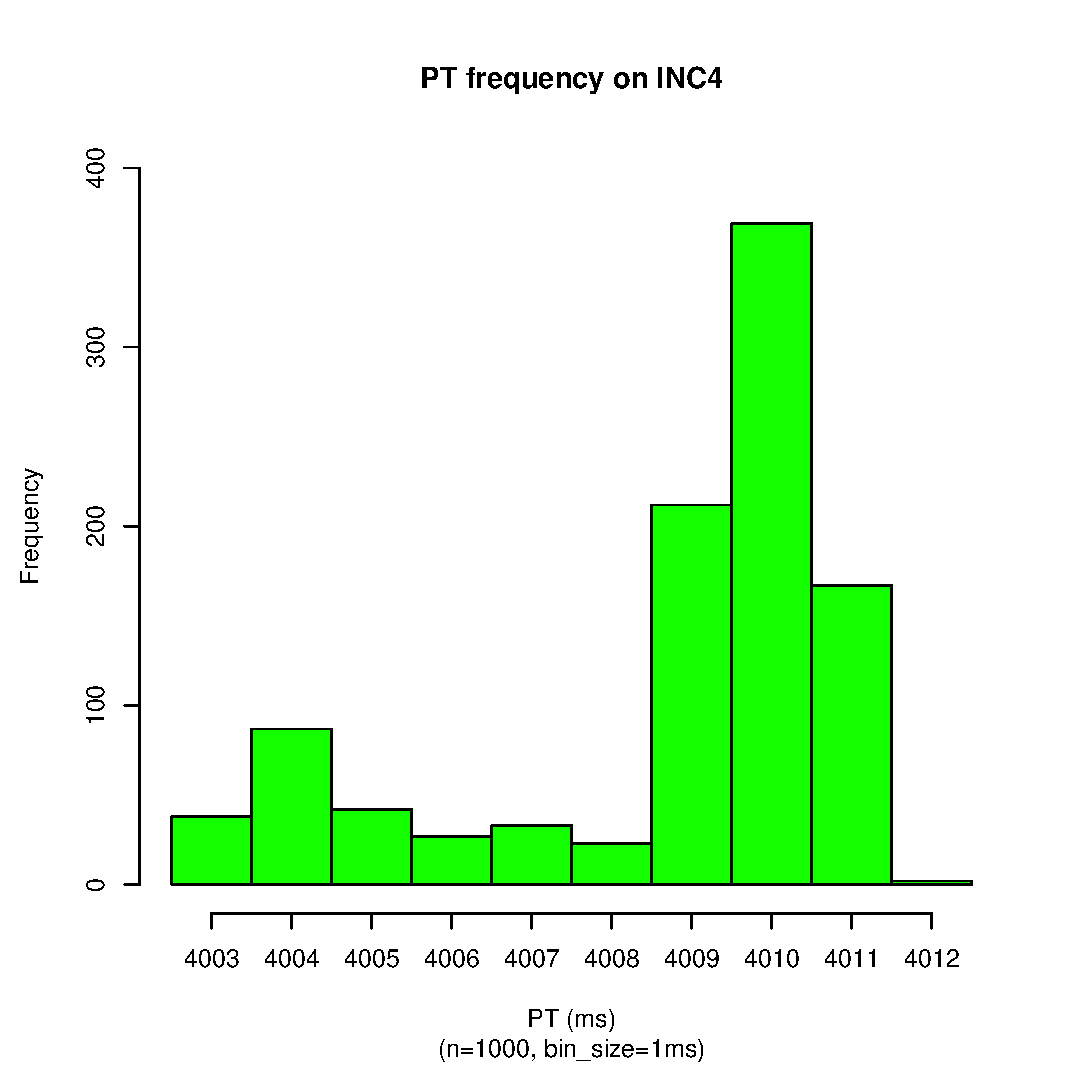
\includegraphics[scale=0.43]{repet_data1/4_sec_pt_hist_v5.eps}
		\label{fig:inc4_r1_hist_v5}
	}
	\subfigure[PT frequency on INC8]{
		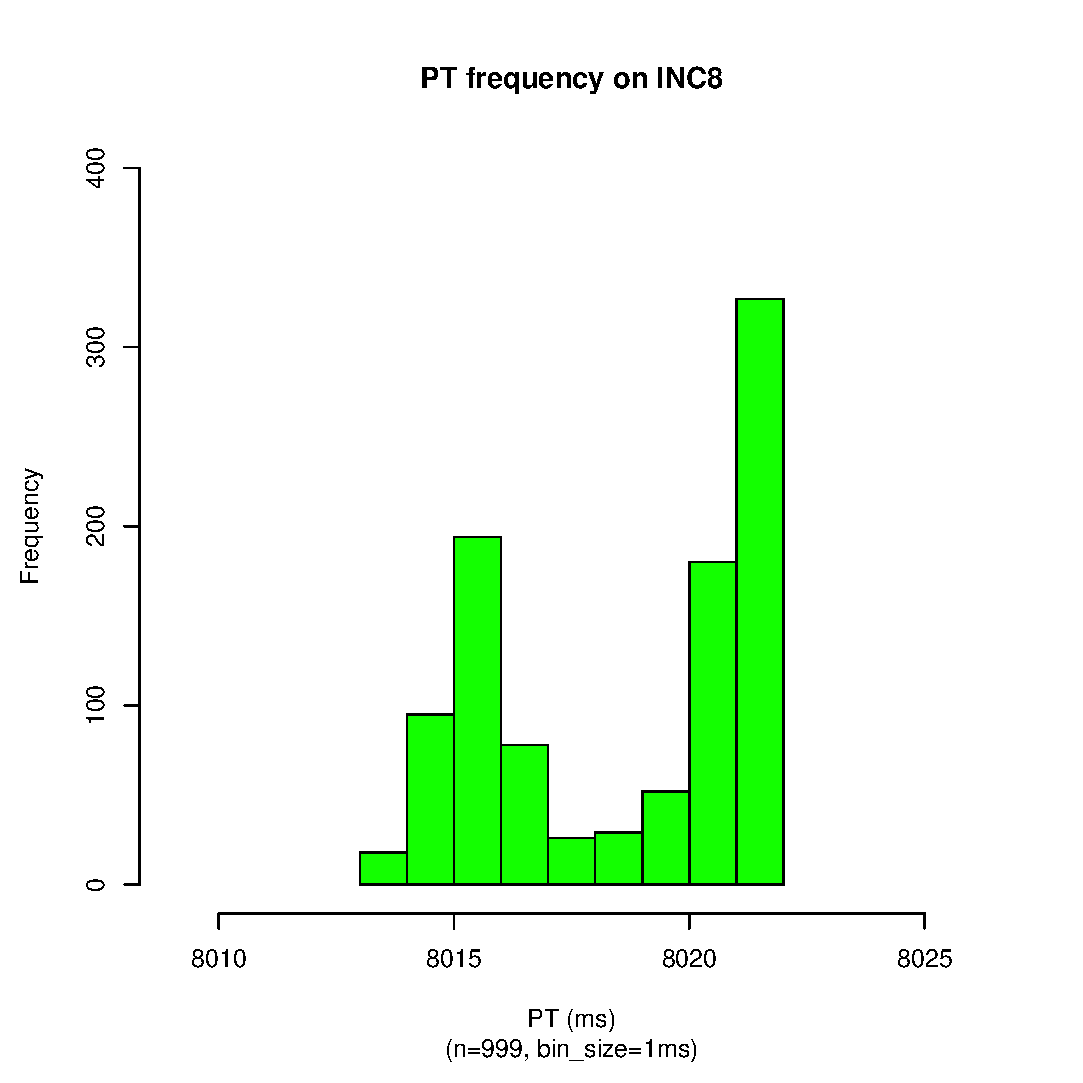
\includegraphics[scale=0.43]{repet_data1/8_sec_pt_hist_v5.eps}
		\label{fig:inc8_r1_hist_v5}
	}
	\caption{PT Histograms of INC1 ... INC8~\label{fig:s9_r1_pt_hist1}}
\end{figure}

\begin{figure}[hp!]
	\centering
	\subfigure[PT frequency on INC16]{
		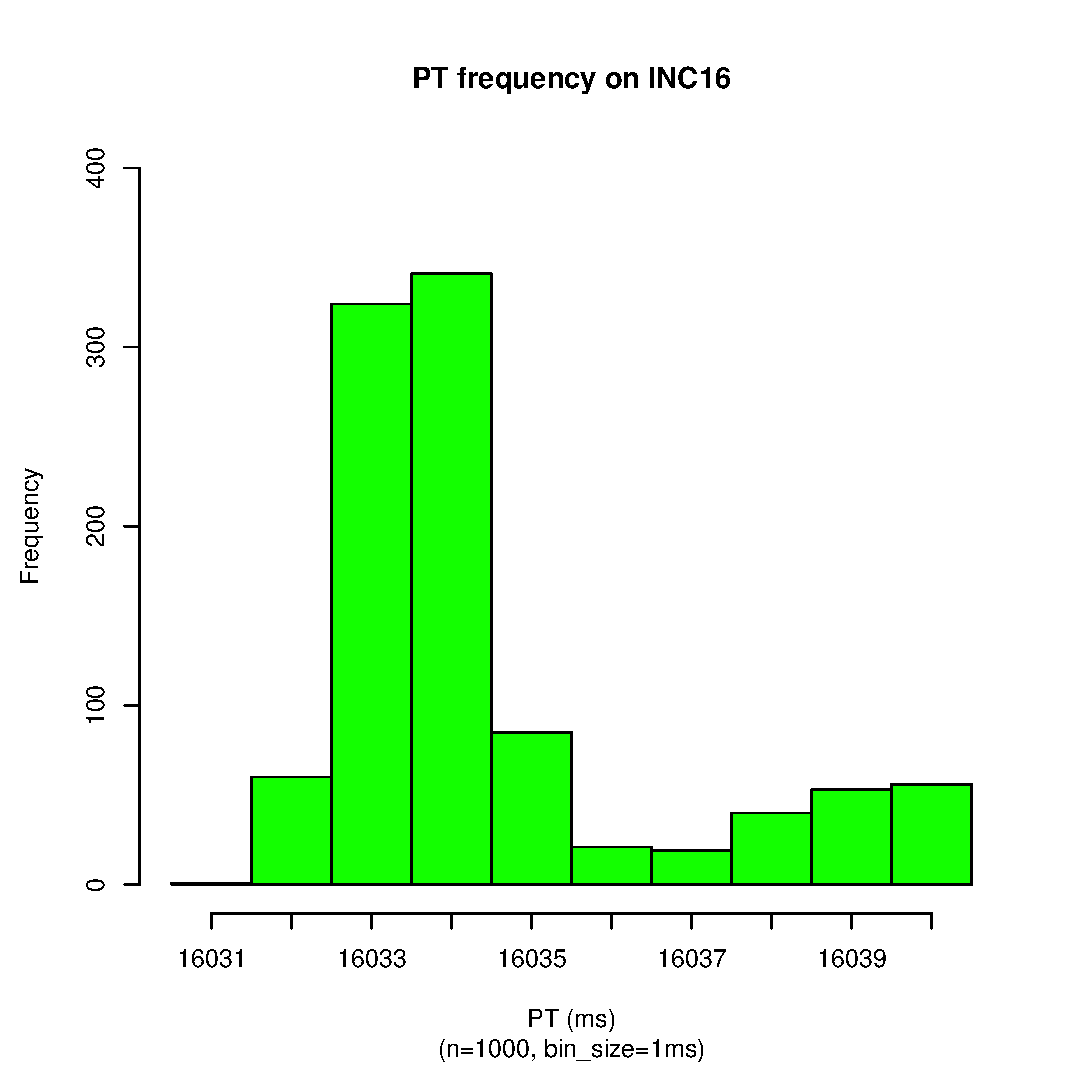
\includegraphics[scale=0.43]{repet_data1/16_sec_pt_hist_v5.eps}
		\label{fig:inc16_r1_hist_v5}
	}
	\subfigure[PT frequency on INC32]{
		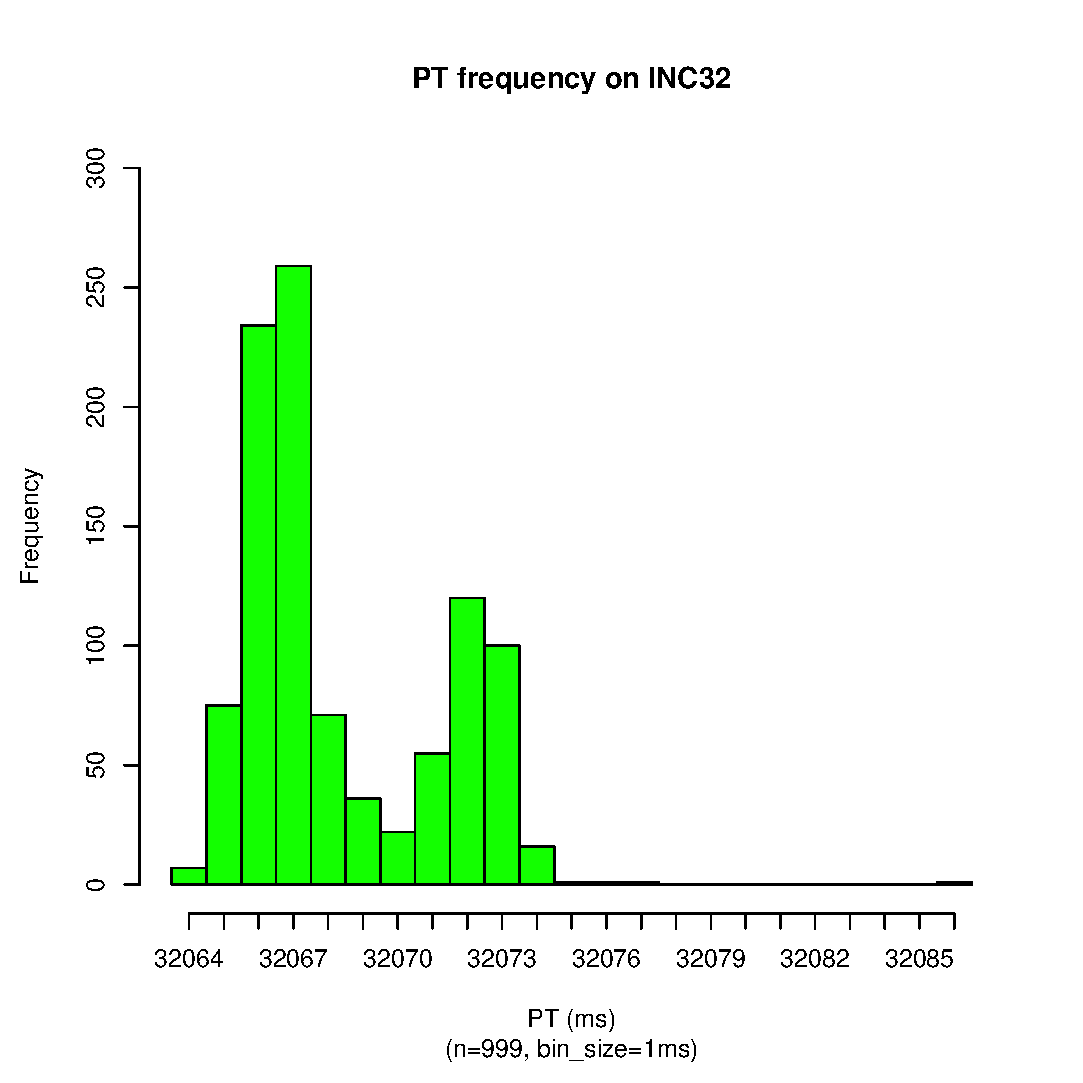
\includegraphics[scale=0.43]{repet_data1/32_sec_pt_hist_v5.eps}
		\label{fig:inc32_r1_hist_v5}
	}
	\subfigure[PT frequency on INC64]{
		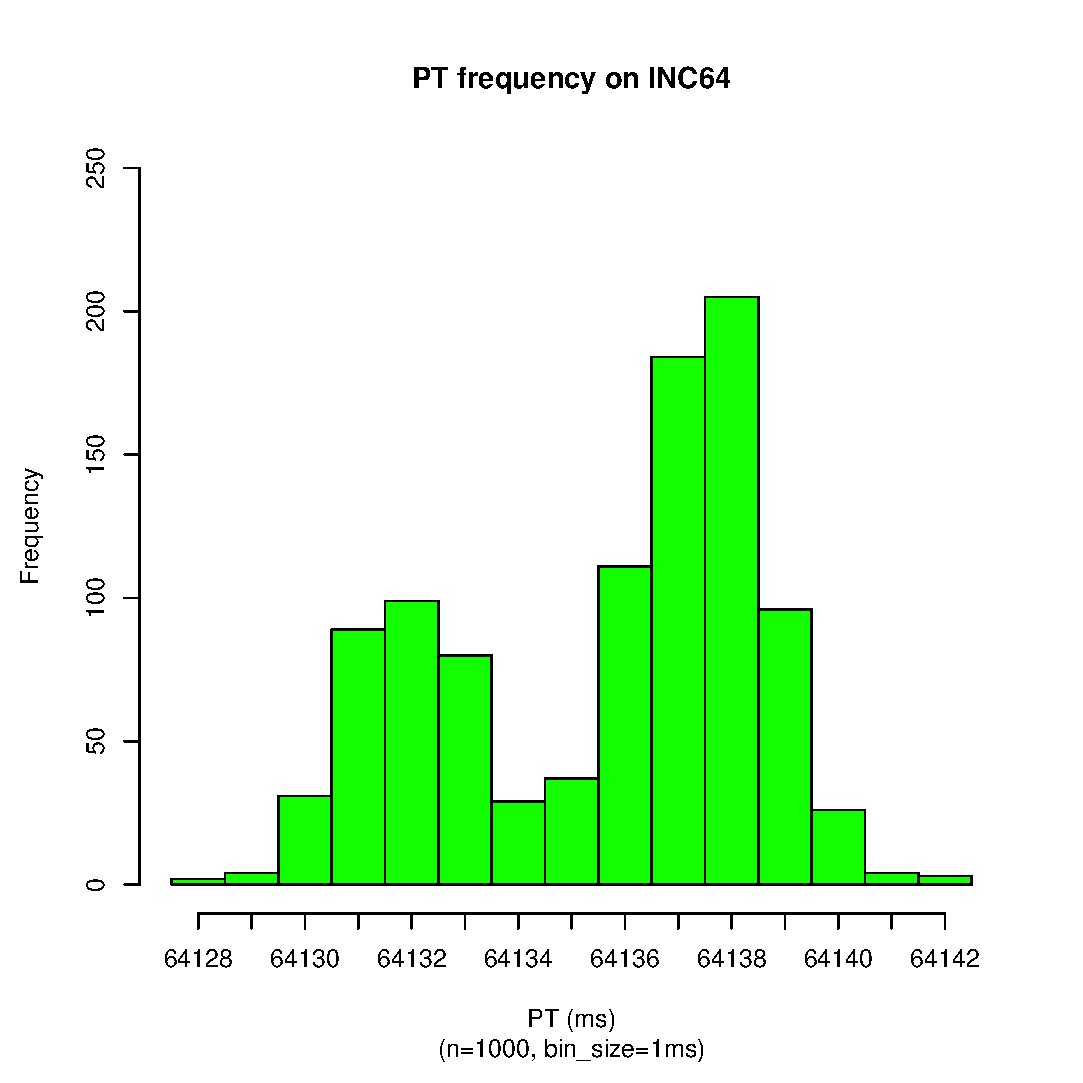
\includegraphics[scale=0.43]{repet_data1/64_sec_pt_hist_v5.eps}
		\label{fig:inc64_r1_hist_v5}
	}
	\caption{PT Histograms of INC16 ... INC64\label{fig:s9_r1_pt_hist2}}
\end{figure}

\begin{figure}[hp!]
	\centering
	\subfigure[PT frequency on INC128]{
		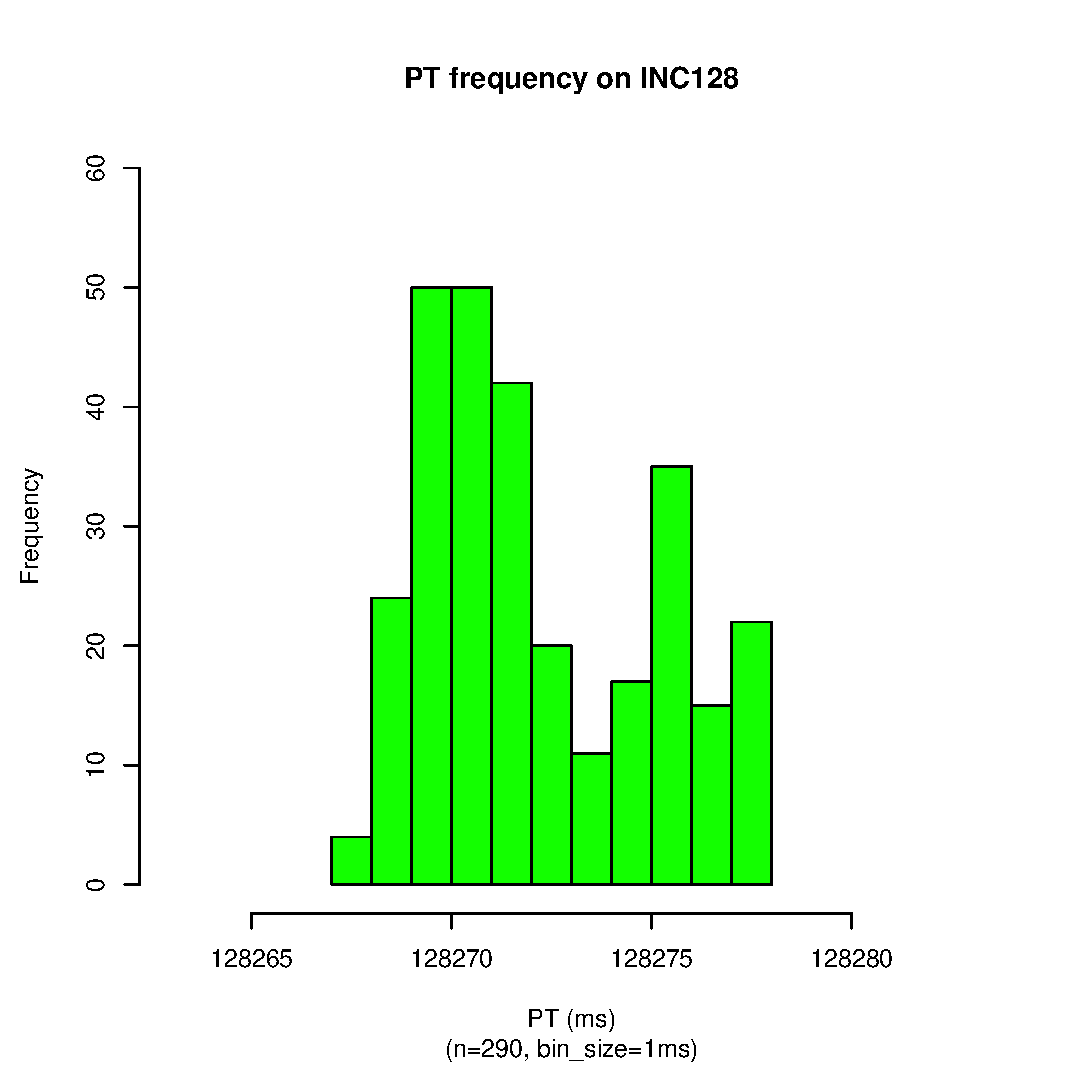
\includegraphics[scale=0.43]{repet_data1/128_sec_pt_hist_v5.eps}
		\label{fig:inc128_r1_hist_v5}
	}
	\subfigure[PT frequency on INC256]{
		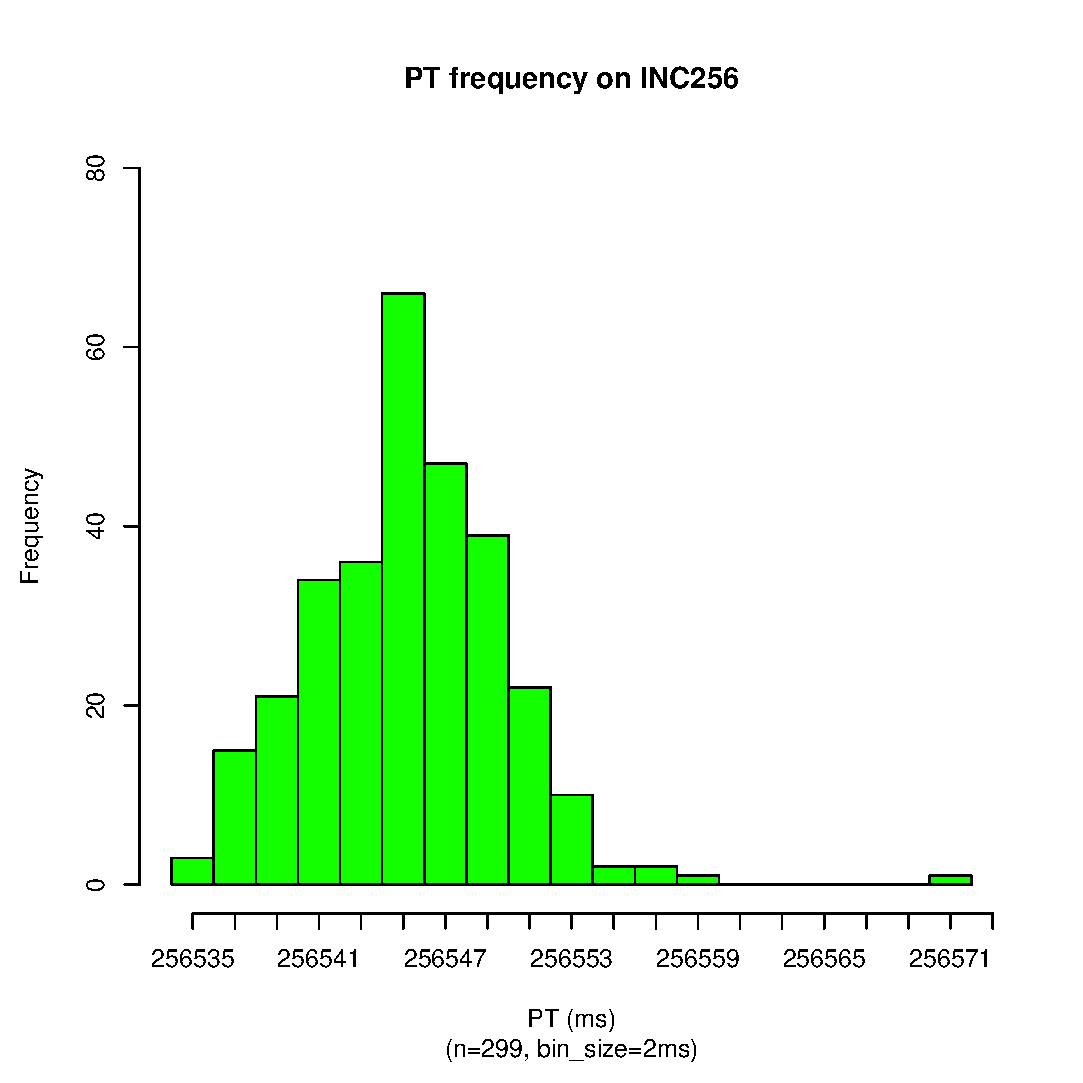
\includegraphics[scale=0.43]{repet_data1/256_sec_pt_hist_v5.eps}
		\label{fig:inc256_r1_hist_v5}
	}
	\subfigure[PT frequency on INC512]{
		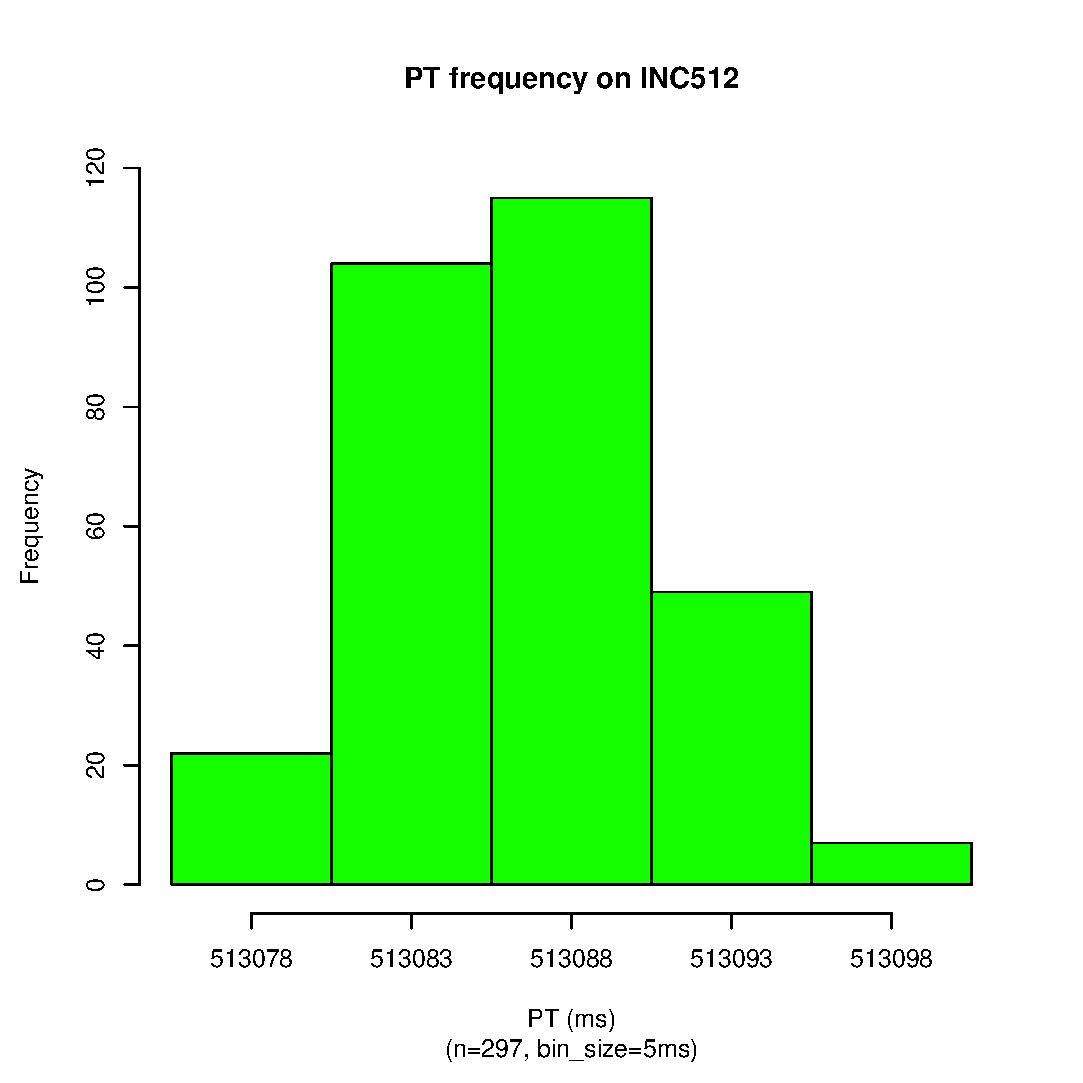
\includegraphics[scale=0.43]{repet_data1/512_sec_pt_hist_v5.eps}
		\label{fig:inc512_r1_hist_v5}
	}
	\subfigure[PT frequency on INC1024]{
		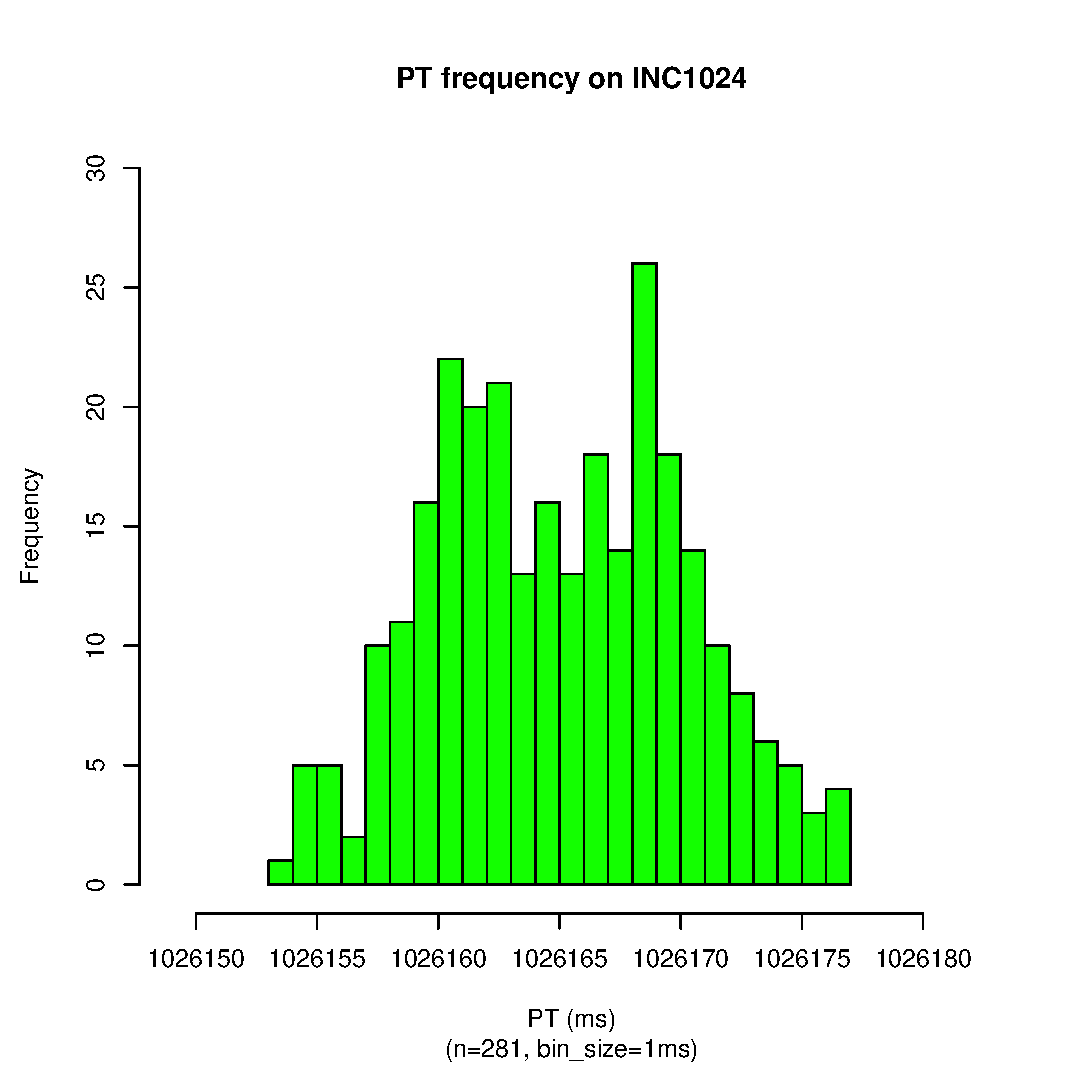
\includegraphics[scale=0.43]{repet_data1/1024_sec_pt_hist_v5.eps}
		\label{fig:inc1024_r1_hist_v5}
	}
	\caption{PT Histograms of INC256 ... INC1024~\label{fig:s9_r1_pt_hist3}}
\end{figure}

\begin{figure}[t]
	\centering
	\subfigure[PT frequency on INC2048]{
		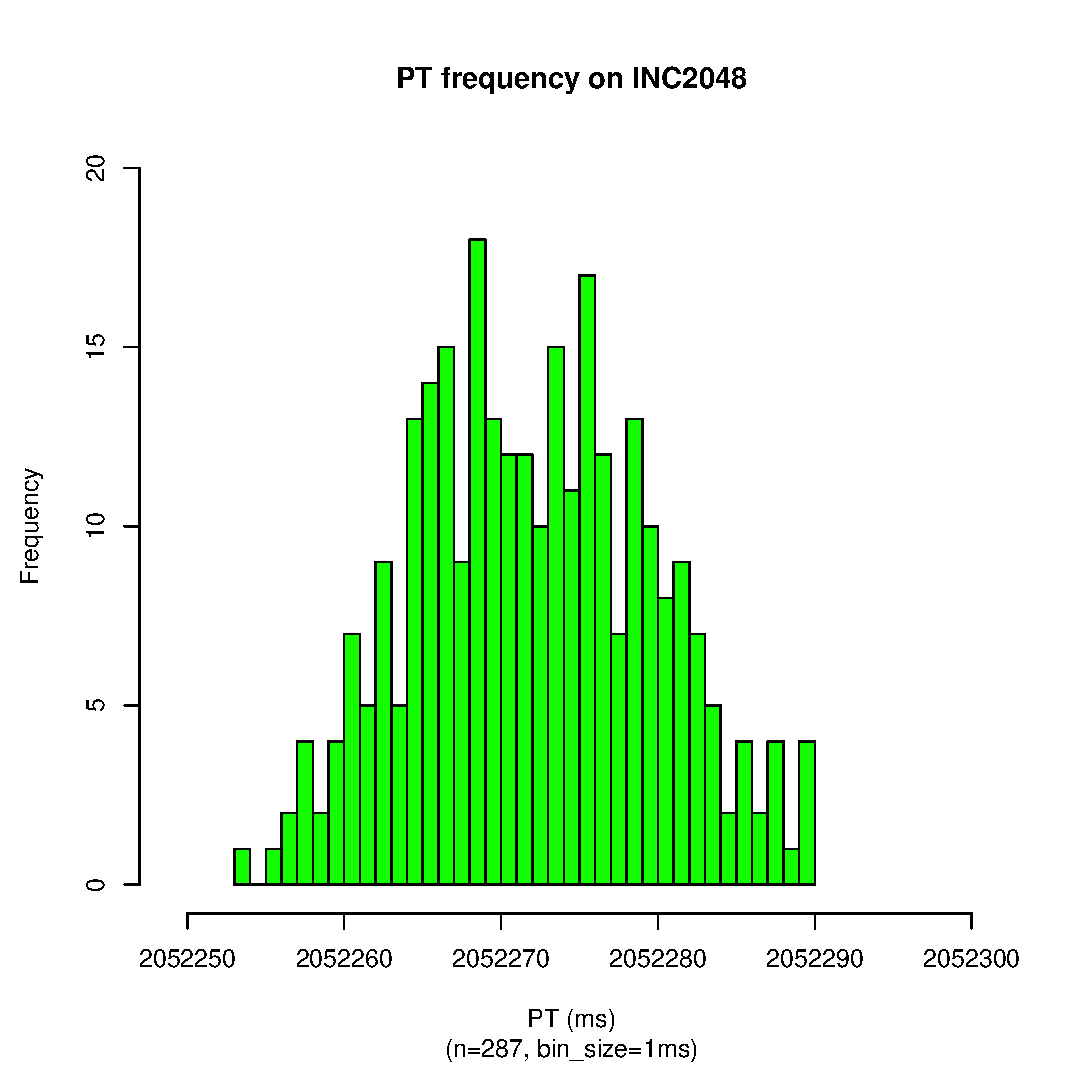
\includegraphics[scale=0.43]{repet_data1/2048_sec_pt_hist_v5.eps}
		\label{fig:inc2048_r1_hist_v5}
	}
	\subfigure[PT frequency on INC4096]{
		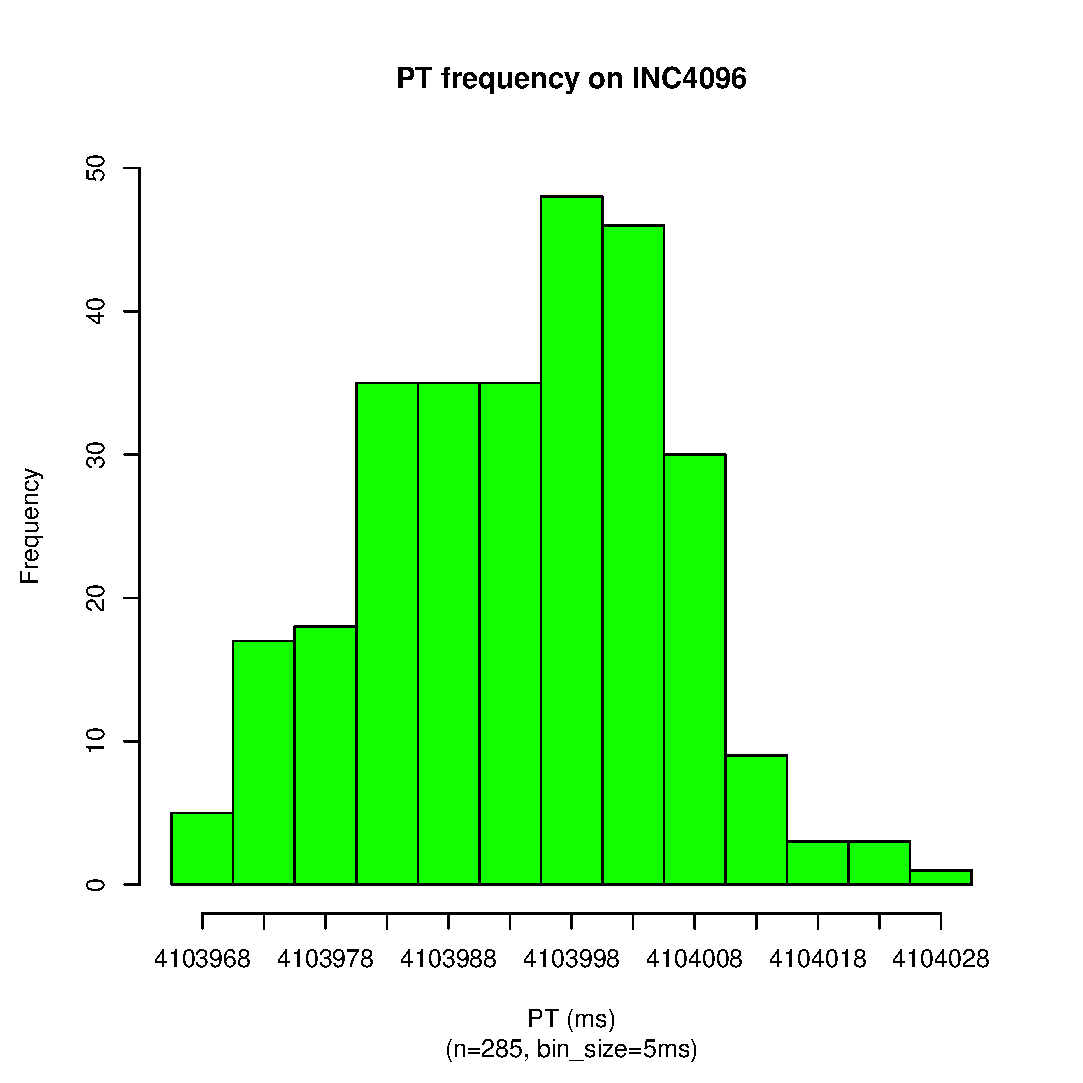
\includegraphics[scale=0.43]{repet_data1/4096_sec_pt_hist_v5.eps}
		\label{fig:inc4096_r1_hist_v5}
	}
	\caption{PT Histograms of INC2048 and INC4096~\label{fig:s9_r1_pt_hist4}}
\end{figure}

\clearpage

\pagebreak
\newpage

\subsection{Additional Histograms}
This section exhibits the histograms of INC with some intermediate task lengths under 256 secs. 
These histograms are intended to investigate where the crossing and merge of two peaks that are consistently observed up to INC128 
happened. Table~\ref{tab:exp_notes4} provides a description of the intermediate runs. 
%and the second run of INC from 8192 seconds to 16384 seconds via EMPv5 with no Step 2.
\begin{table}[h]
\begin{center}
\begin{tabular}{|p{2cm}|p{3cm}|p{3cm}|p{4cm}|p{3.5cm}|} \hline
Machine & Task Length (sec) & Description & Experiment Period & Relevant \linebreak Histograms\\ \hline
{\tt sodb9} &  INC96$\sim$INC256 & 1000 samples, each & 2017-05-24 $\sim$ 2017-06-06 & 
Figs.~\ref{fig:ut_hist3}, \ref{fig:inc224_ut_hist}, and~\ref{fig:inc256_ut_hist}\\ \hline
					&  INC3, 6, 12, 24, 48, 72, 80, 88, 104, 112, and 120 & 1000 samples, each & 2017-06-07 $\sim$ 2017-06-16 & Figs.~\ref{fig:inc3_ut_hist}, ~\ref{fig:inc6_ut_hist}, ~\ref{fig:inc12_ut_hist}, ~\ref{fig:inc24_ut_hist},
~\ref{fig:inc48_ut_hist}, ~\ref{fig:inc72_ut_hist}, ~\ref{fig:inc80_ut_hist}, ~\ref{fig:inc88_ut_hist}, ~\ref{fig:inc104_ut_hist},~\ref{fig:inc112_ut_hist}, and~\ref{fig:inc120_ut_hist}\\ \hline
\end{tabular}
\end{center}
\vspace{-.2in}
\caption{Notes on experiment runs used for histograms\label{tab:exp_notes4}}
\end{table}

\subsubsection{ET}
Not available at this point, due to the labshelf server's unavailability for the time being.

\pagebreak

\subsubsection{PT}
%The histograms of INC1 through INC4096 are 
%the same as those of Figures~\ref{fig:s9_r1_pt_hist1},~\ref{fig:s9_r1_pt_hist2},~\ref{fig:s9_r1_pt_hist3}, and~\ref{fig:s9_r1_pt_hist4}. 

\begin{figure}[hp!]
	\centering
	\subfigure[PT frequency on INC3]{
		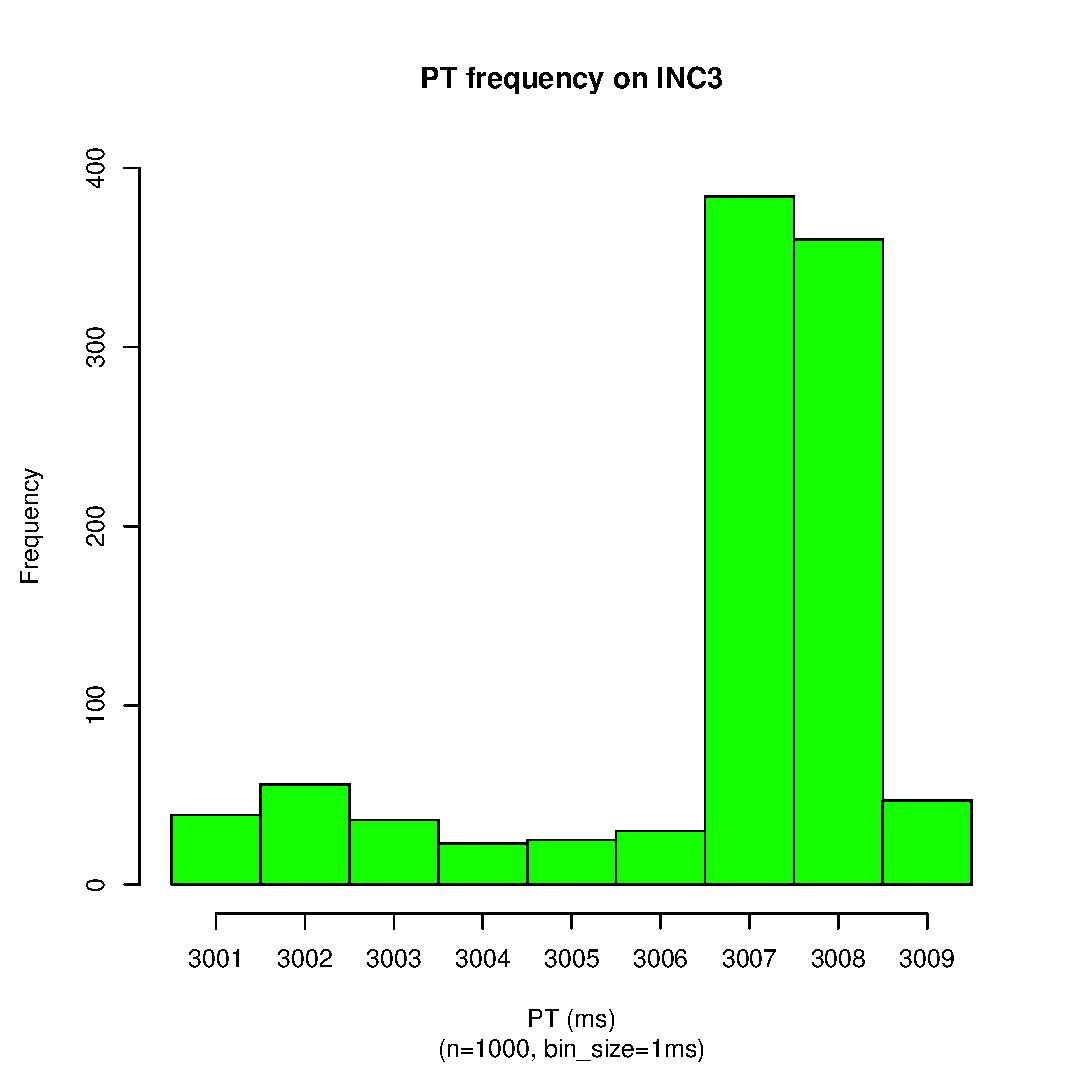
\includegraphics[scale=0.43]{u_s_time/3_sec_pt_hist.eps}
		\label{fig:inc3_pt_hist}
	}
	\subfigure[PT frequency on INC6]{
		\includegraphics[scale=0.43]{u_s_time/6_sec_pt_hist.eps}
		\label{fig:inc6_pt_hist}
	}
	\subfigure[PT frequency on INC12]{
		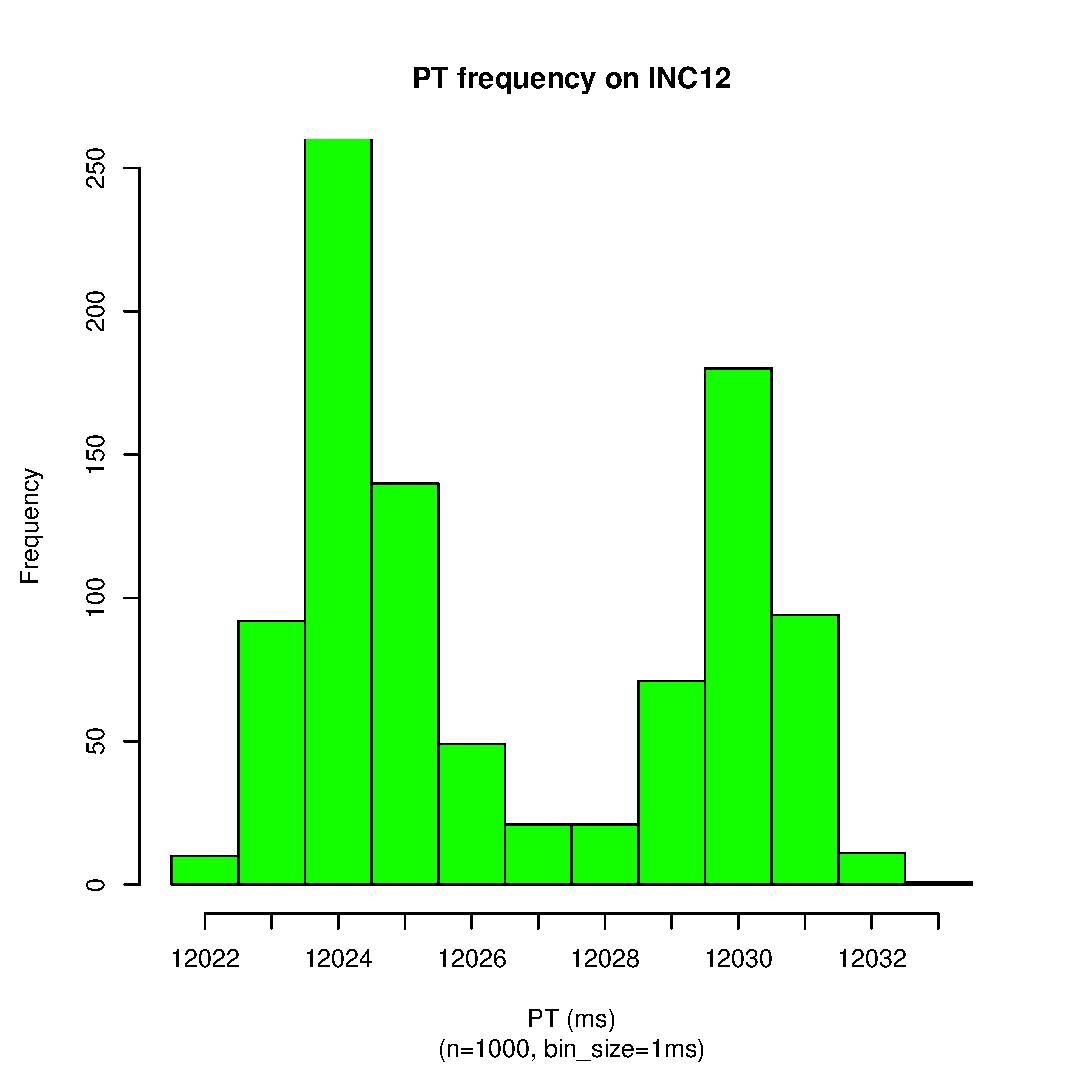
\includegraphics[scale=0.43]{u_s_time/12_sec_pt_hist.eps}
		\label{fig:inc12_pt_hist}
	}
	\subfigure[PT frequency on INC24]{
		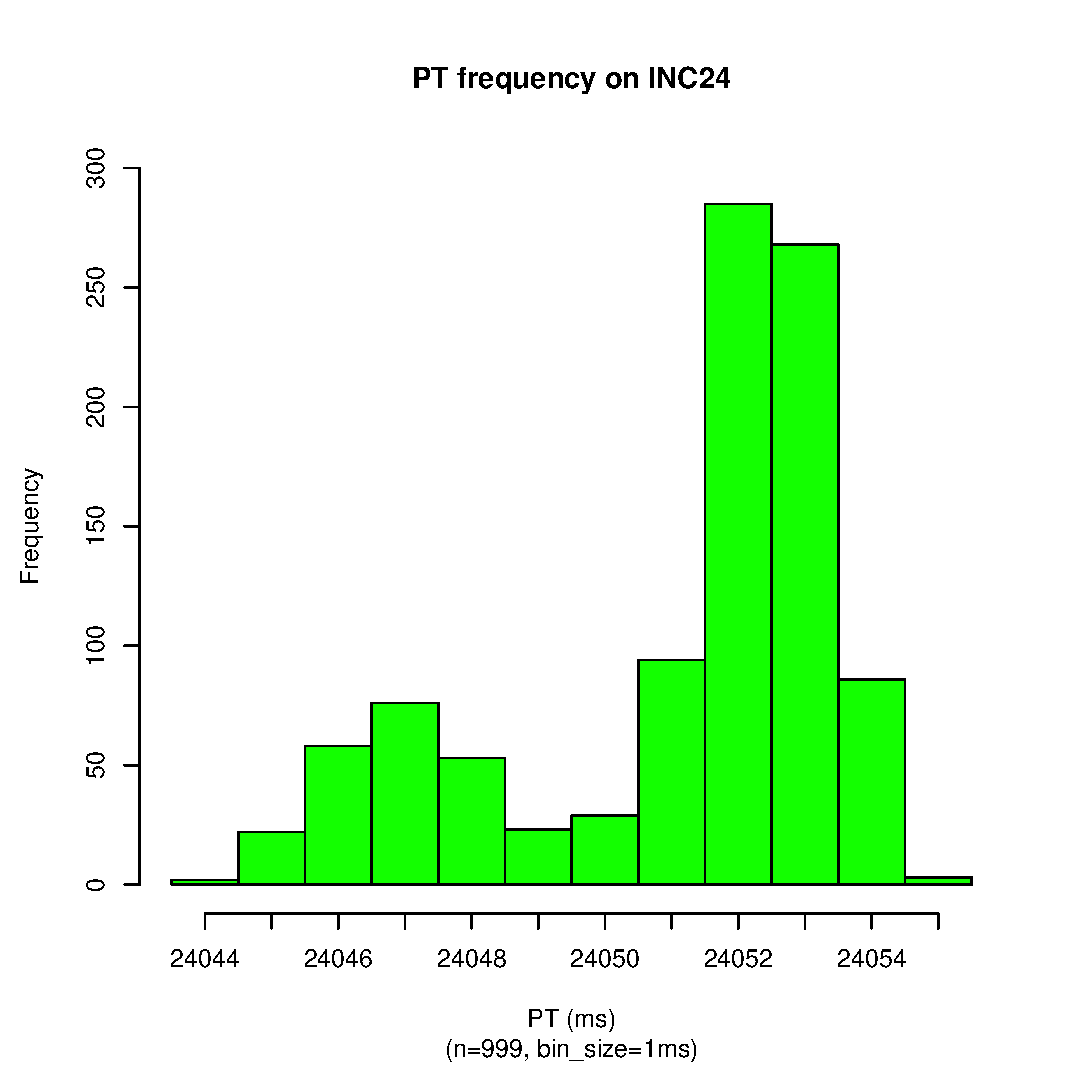
\includegraphics[scale=0.43]{u_s_time/24_sec_pt_hist.eps}
		\label{fig:inc24_pt_hist}
	}
	\caption{PT Histograms of INC3 ... INC24~\label{fig:new_pt_hist1}}
\end{figure}

\pagebreak
\newpage

\begin{figure}[hp!]
	\centering
	\subfigure[PT frequency on INC48]{
		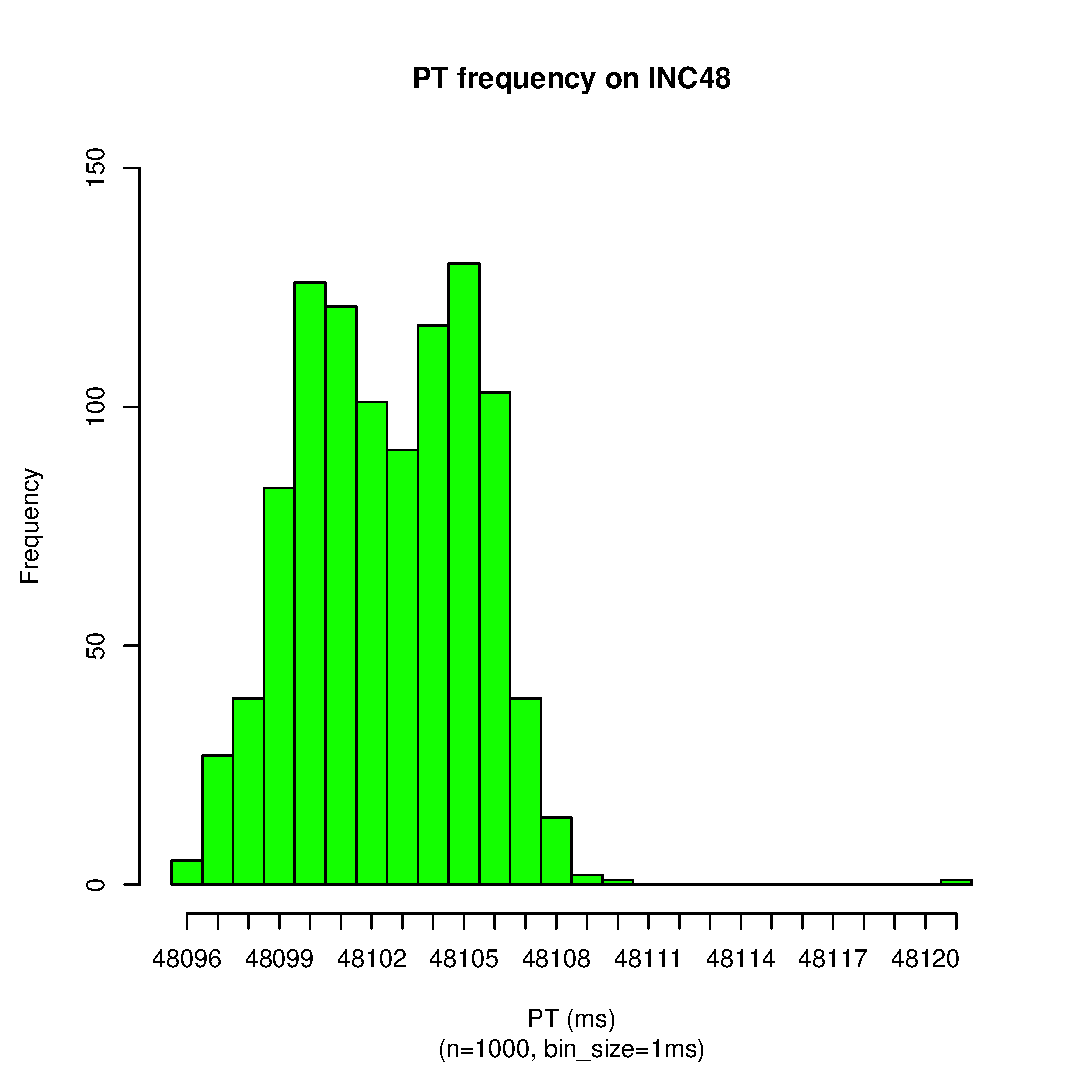
\includegraphics[scale=0.43]{u_s_time/48_sec_pt_hist.eps}
		\label{fig:inc48_pt_hist}
	}
	\subfigure[PT frequency on INC72]{
		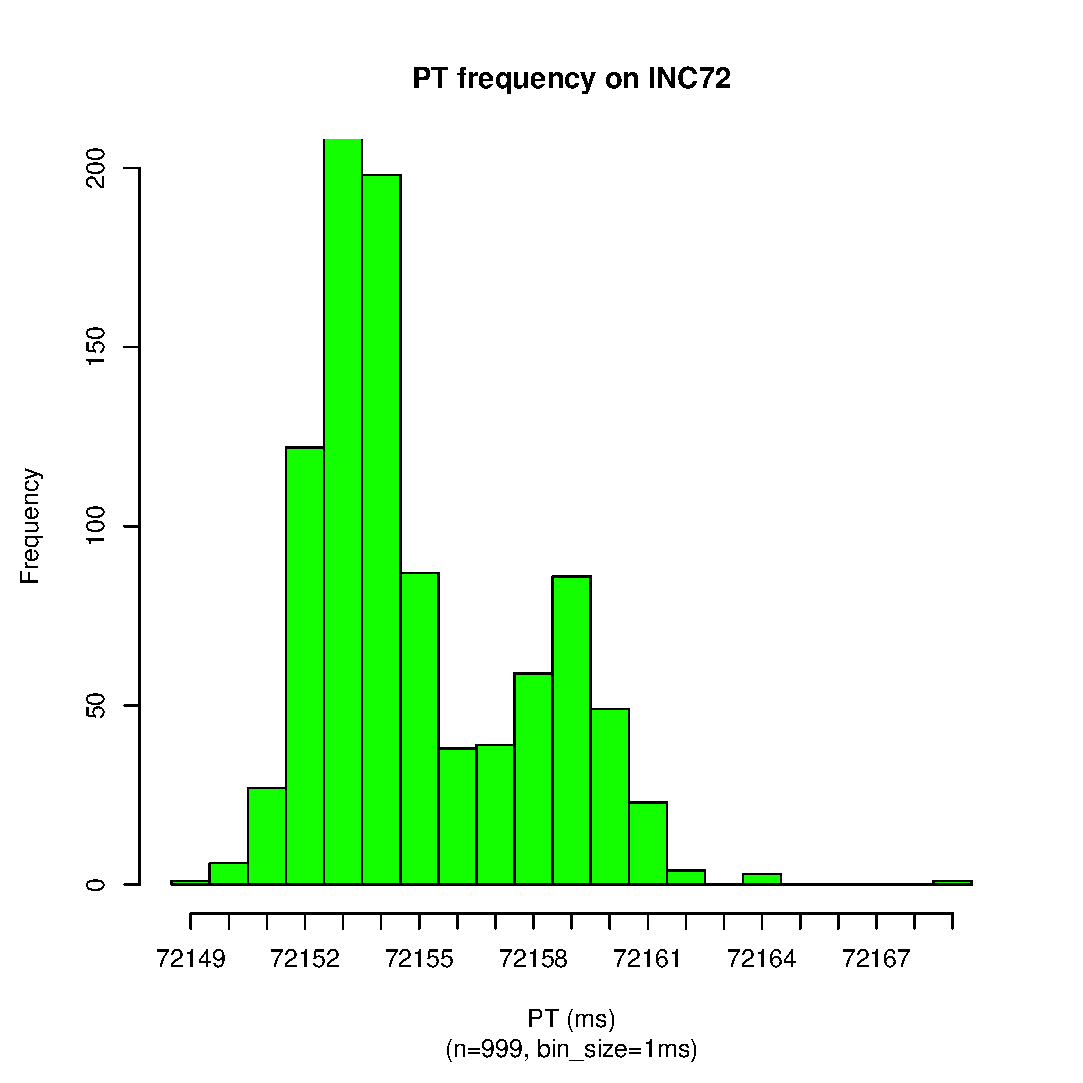
\includegraphics[scale=0.43]{u_s_time/72_sec_pt_hist.eps}
		\label{fig:inc72_pt_hist}
	}
	\subfigure[PT frequency on INC80]{
		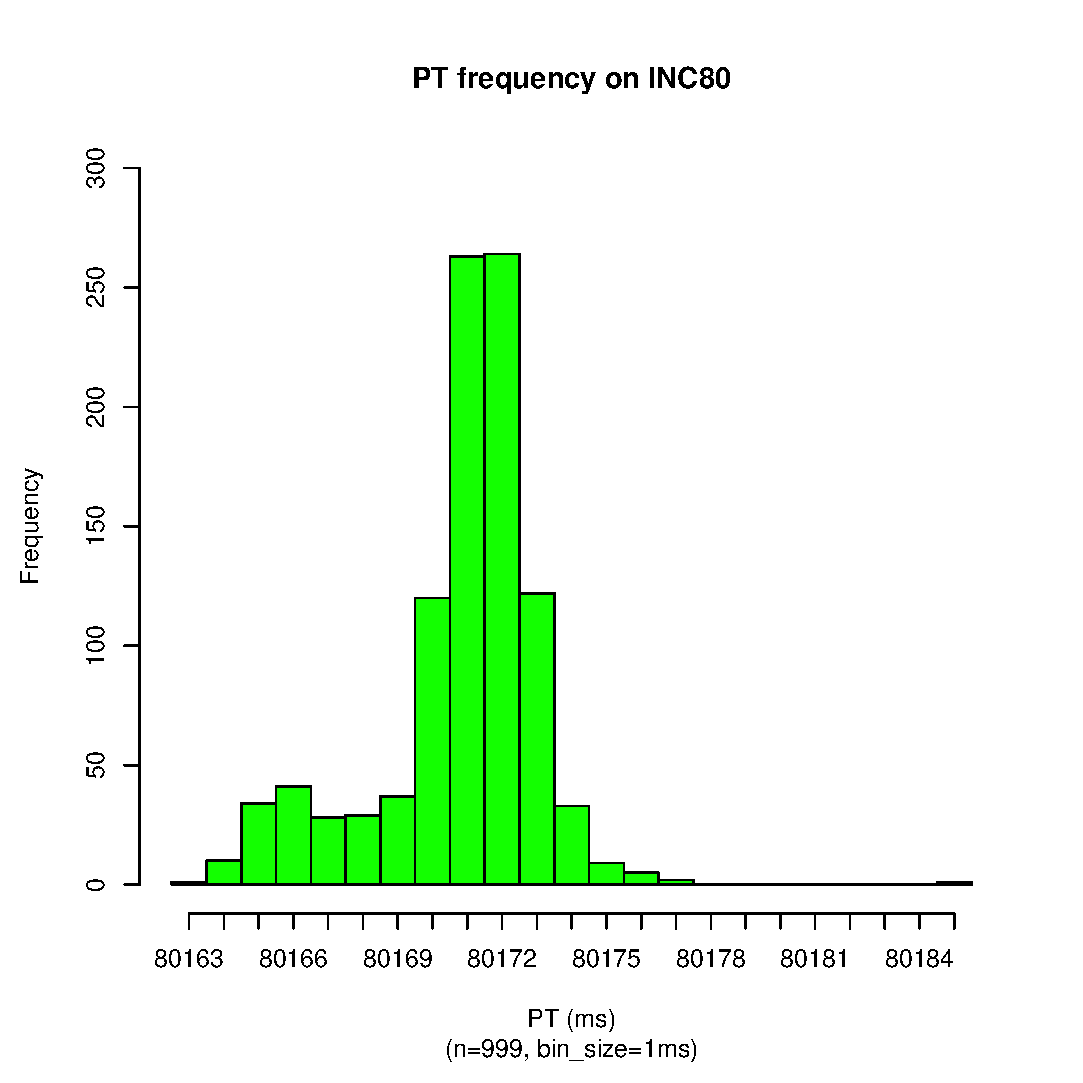
\includegraphics[scale=0.43]{u_s_time/80_sec_pt_hist.eps}
		\label{fig:inc80_pt_hist}
	}
	\subfigure[PT frequency on INC88]{
		\includegraphics[scale=0.43]{u_s_time/88_sec_pt_hist.eps}
		\label{fig:inc88_pt_hist}
	}
	\caption{PT Histograms of INC48 ... INC88~\label{fig:new_pt_hist2}}
\end{figure}

\pagebreak
\newpage

\begin{figure}[hp!]
	\centering
	\subfigure[PT frequency on INC96]{
		\includegraphics[scale=0.43]{u_s_time/96_sec_pt_hist.eps}
		\label{fig:inc96_pt_hist}
	}
	\subfigure[PT frequency on INC104]{
		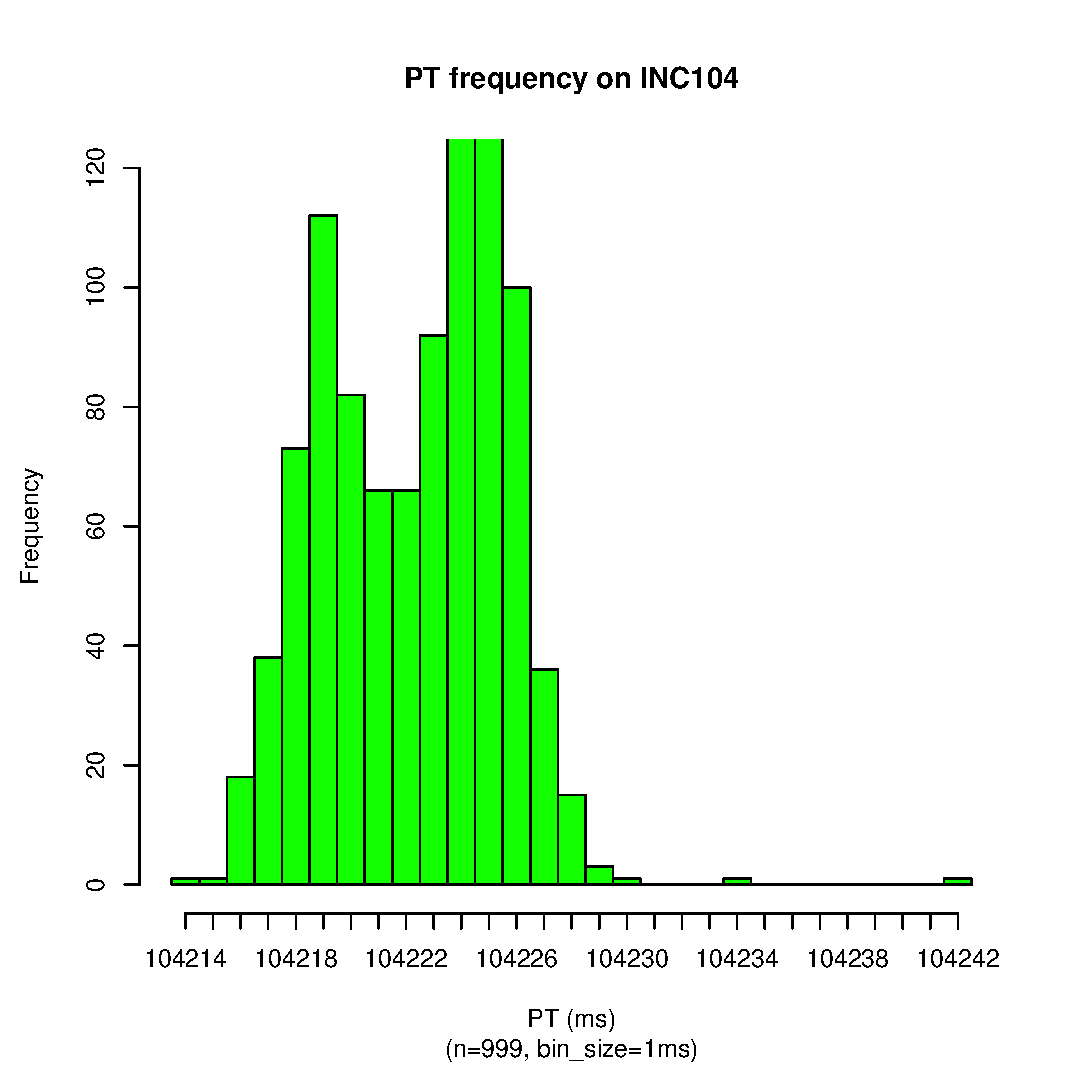
\includegraphics[scale=0.43]{u_s_time/104_sec_pt_hist.eps}
		\label{fig:inc104_pt_hist}
	}
	\subfigure[PT frequency on INC112]{
		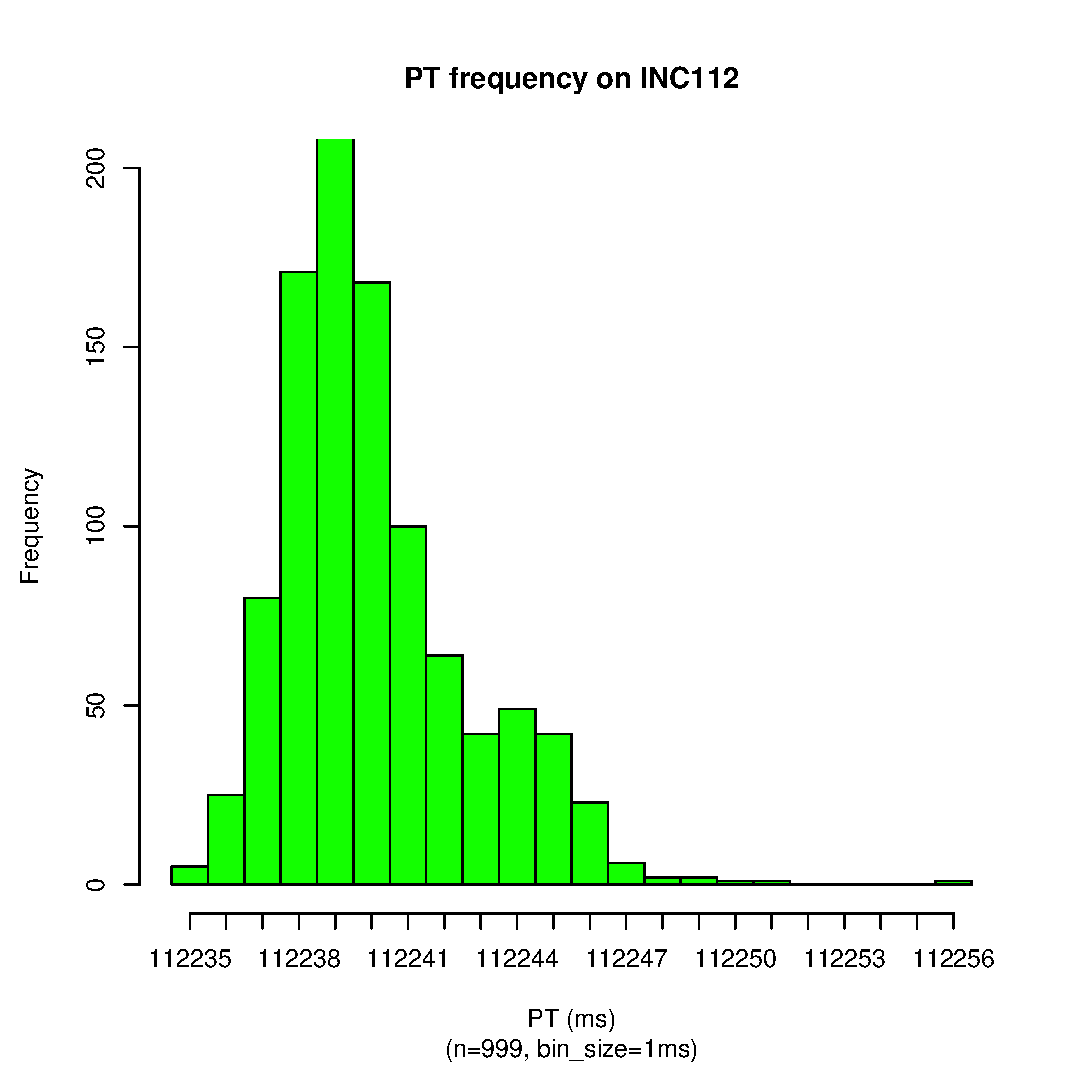
\includegraphics[scale=0.43]{u_s_time/112_sec_pt_hist.eps}
		\label{fig:inc112_pt_hist}
	}
	\subfigure[PT frequency on INC120]{
		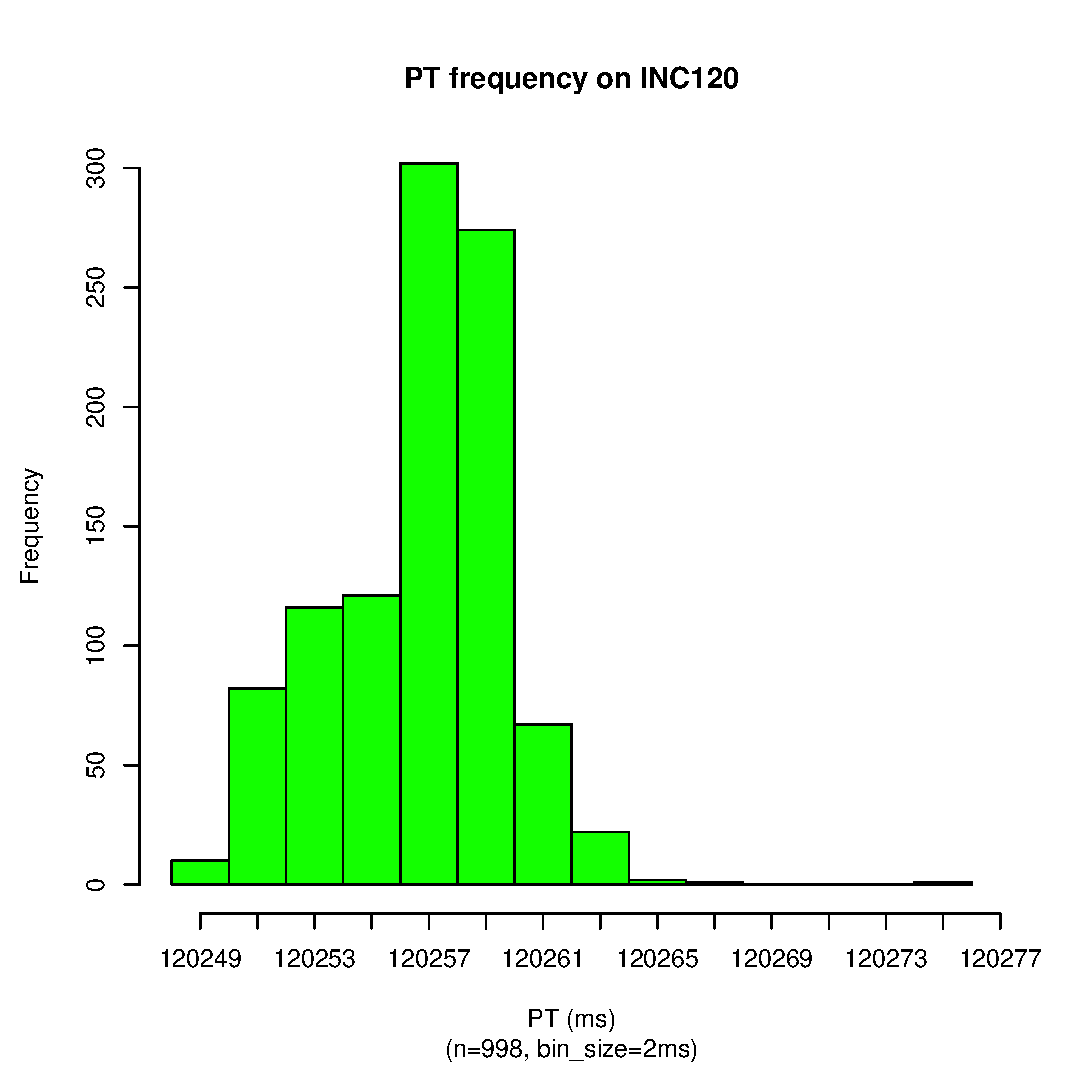
\includegraphics[scale=0.43]{u_s_time/120_sec_pt_hist.eps}
		\label{fig:inc120_pt_hist}
	}
	\caption{PT Histograms of INC96 ... INC120~\label{fig:new_pt_hist3}}
\end{figure}

\pagebreak
\newpage

\begin{figure}[hp!]
	\centering
	\subfigure[PT frequency on INC160]{
		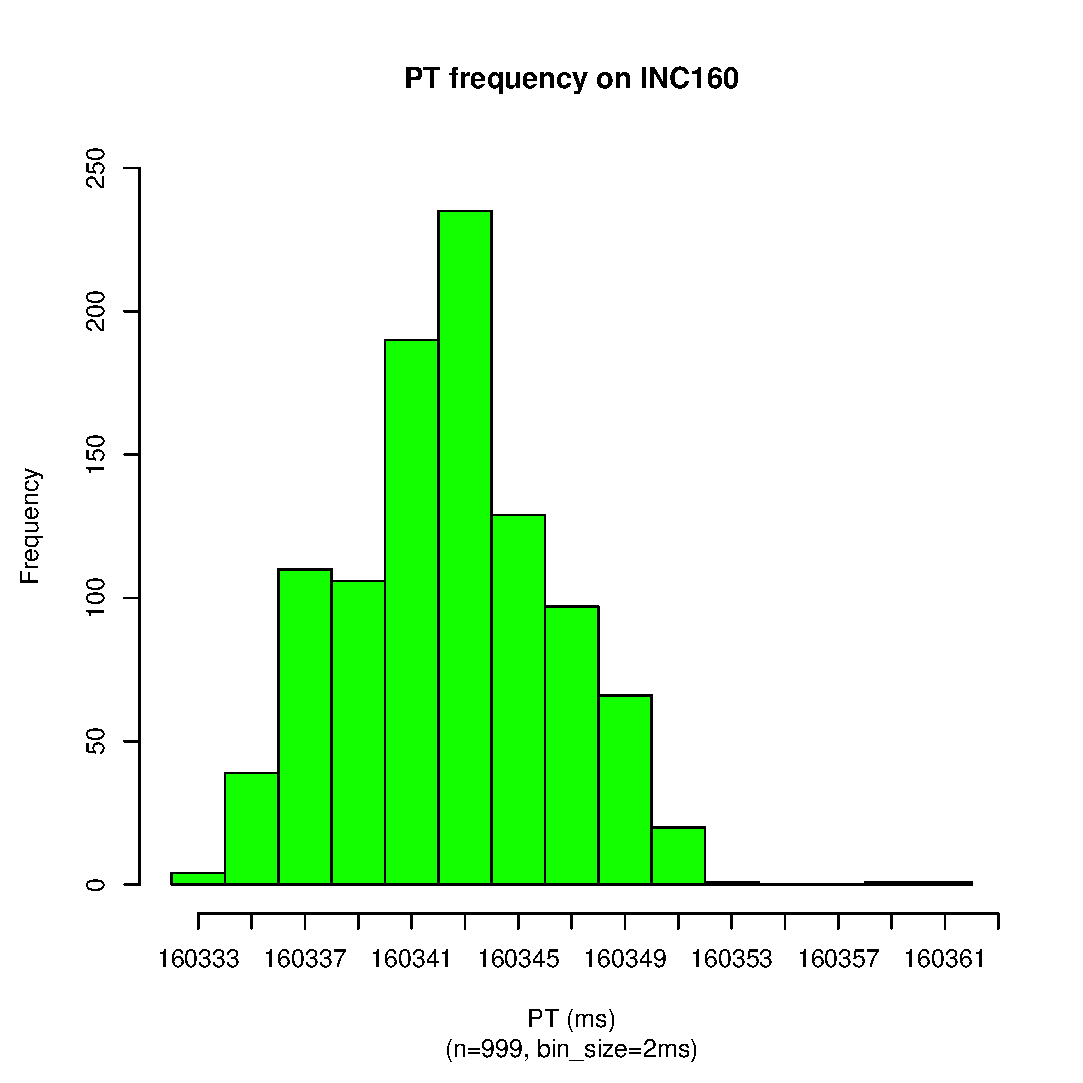
\includegraphics[scale=0.43]{u_s_time/160_sec_pt_hist.eps}
		\label{fig:inc160_pt_hist}
	}
	\subfigure[PT frequency on INC192]{
		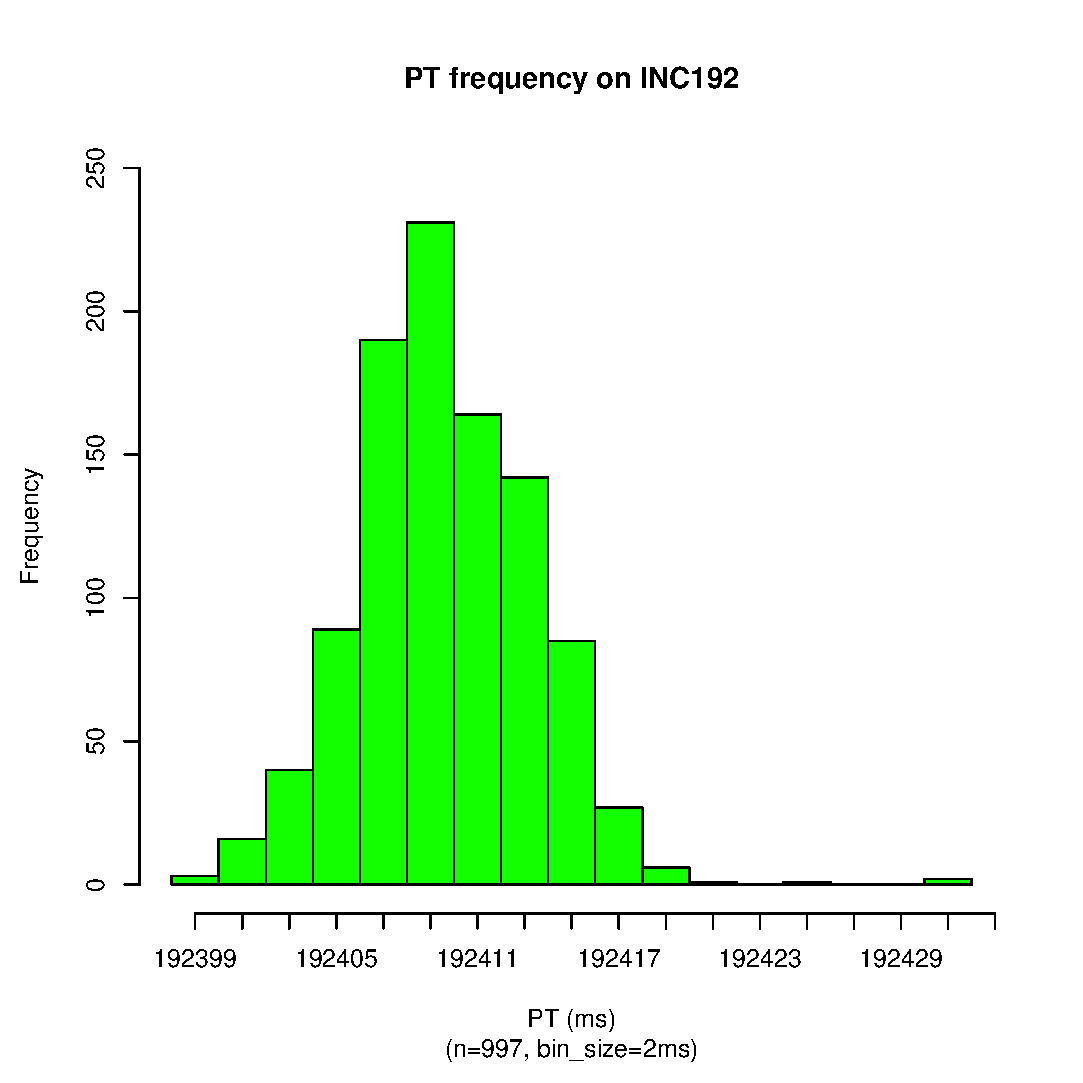
\includegraphics[scale=0.43]{u_s_time/192_sec_pt_hist.eps}
		\label{fig:inc192_pt_hist}
	}
	\subfigure[PT frequency on INC224]{
		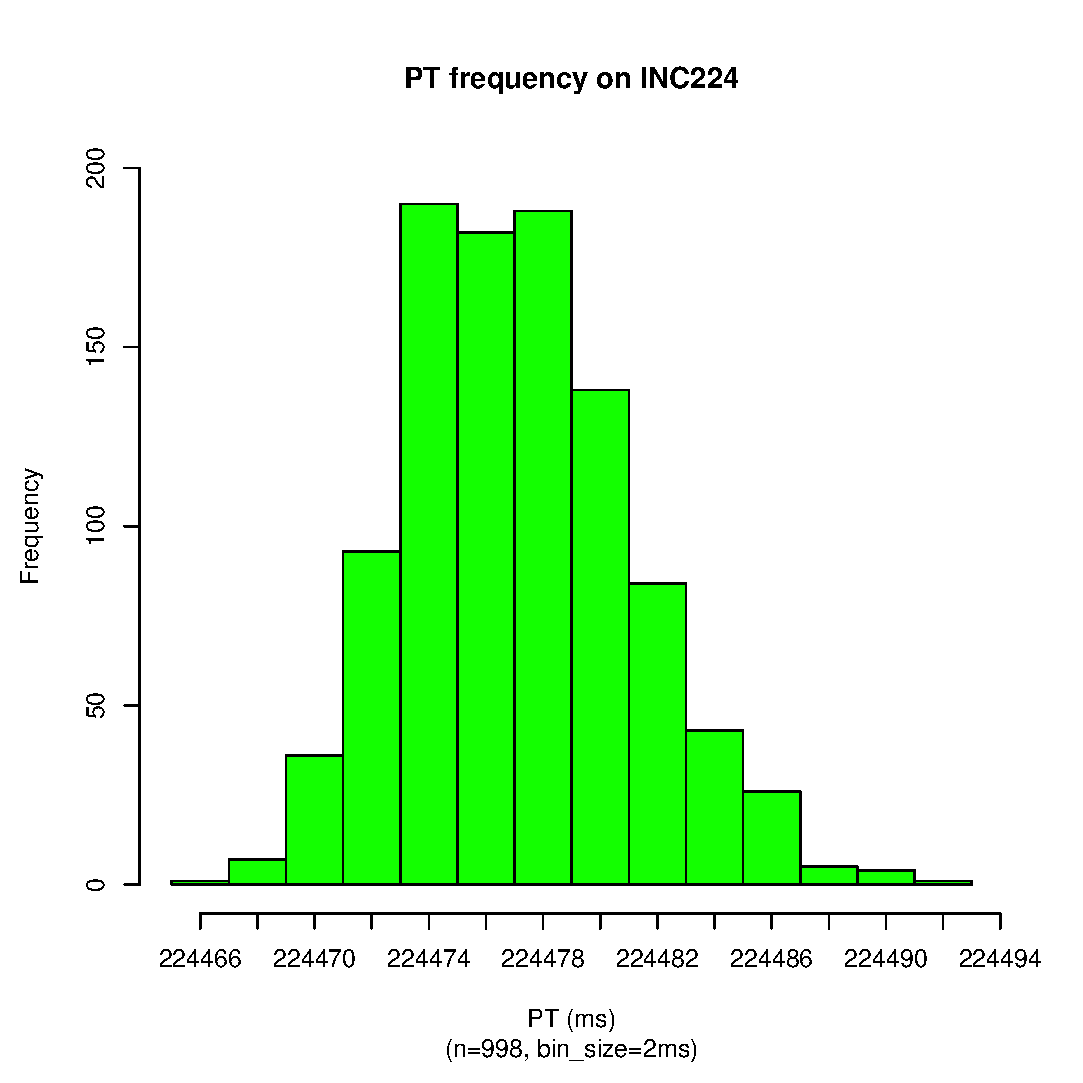
\includegraphics[scale=0.43]{u_s_time/224_sec_pt_hist.eps}
		\label{fig:inc224_pt_hist}
	}
	\caption{PT Histograms of INC169 ... INC224~\label{fig:new_pt_hist4}}
\end{figure}

\pagebreak
\newpage

\subsection{Summary}

\paragraph{Stacked Histograms in a 3D Plot:}
Figure~\ref{fig:hist3d} represents a 3D plot of collecting the histograms of PT 
exhibited in Section~\ref{sec:first_run}. 
Note that the histograms from the task lengths of 8192 and 16384 seconds 
to be shown in Figures~\ref{fig:inc8192_r2_hist_v5} and~\ref{fig:inc16384_r2_hist_v5}. 
are brought into Figure~\ref{fig:hist3d} for completeness. The x-, y-, z-axes 
indicate the normalized PT ranging from 0 to 100, task length in log scale, 
and relative frequency of each histogram, such that for each INC 
it is scaled from 0 (the shortest) to 100 (the highest). 

\begin{figure}[htp!]
%\vspace{-.3in}
	\centering
	%\includegraphics[scale=0.6,angle=270]{u_s_time/3d_plot.eps}\label{fig:3d_plot}
	%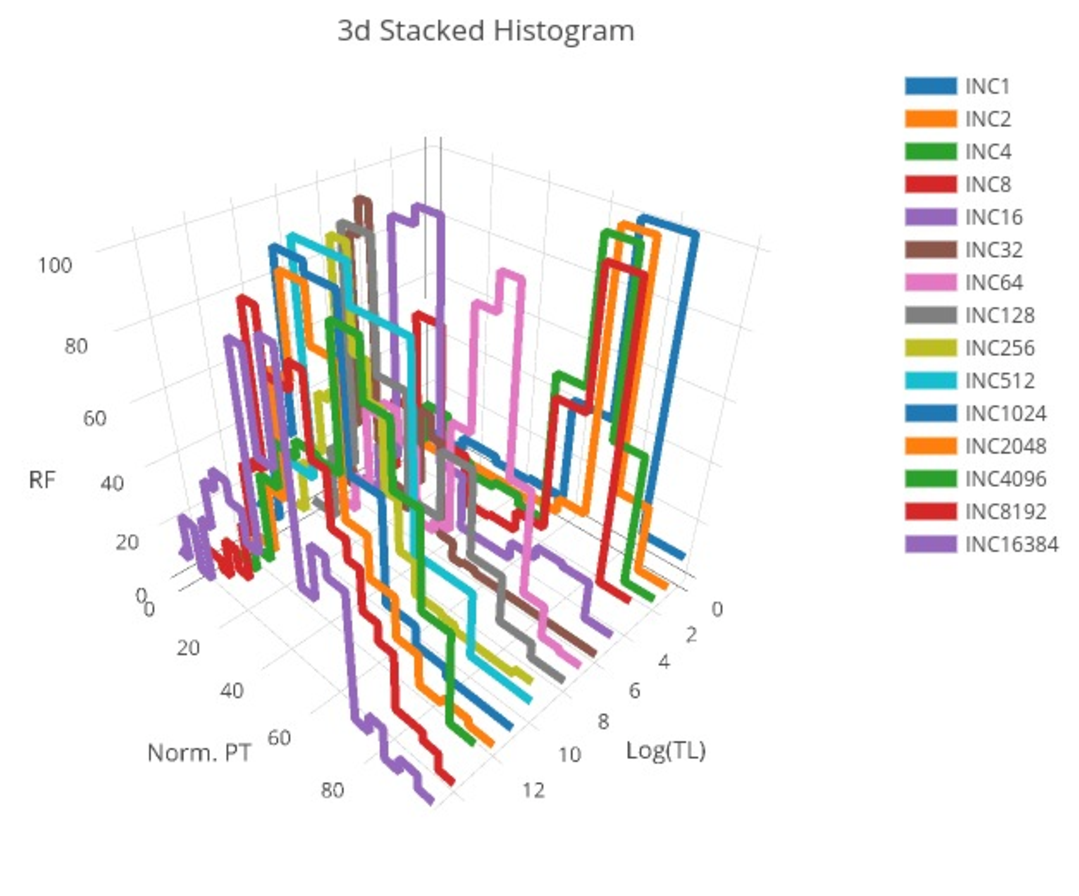
\includegraphics[scale=0.6]{u_s_time/new_3d_plot}\label{fig:3d_plot}
	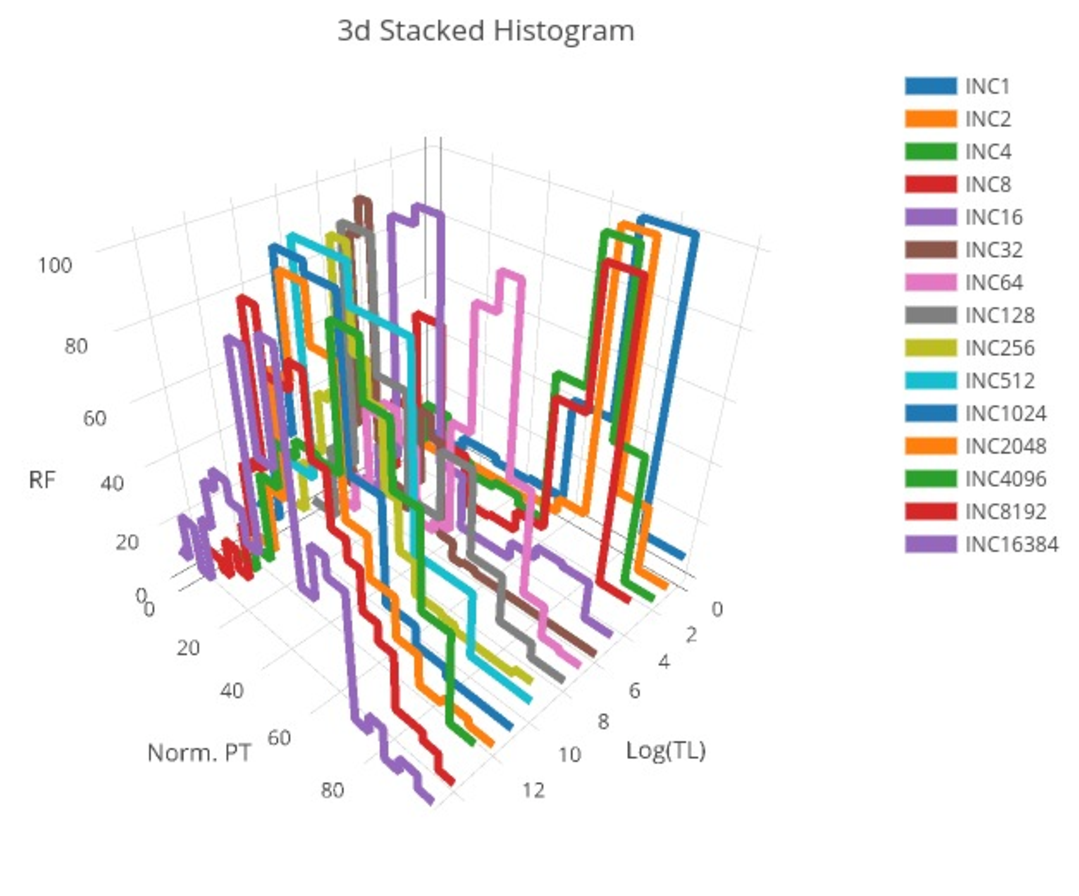
\includegraphics[scale=1]{u_s_time/new_3d_plot}\label{fig:3d_plot}
	\caption{3D histograms on INC~\label{fig:hist3d}}
\end{figure}

\pagebreak
\clearpage
Figure~\ref{fig:hist3d_u} represents a 3D plot of collecting the histograms of user time only
exhibited in Section~\ref{sec:first_run}. 
\begin{figure}[htp!]
%\vspace{-.3in}
	\centering
	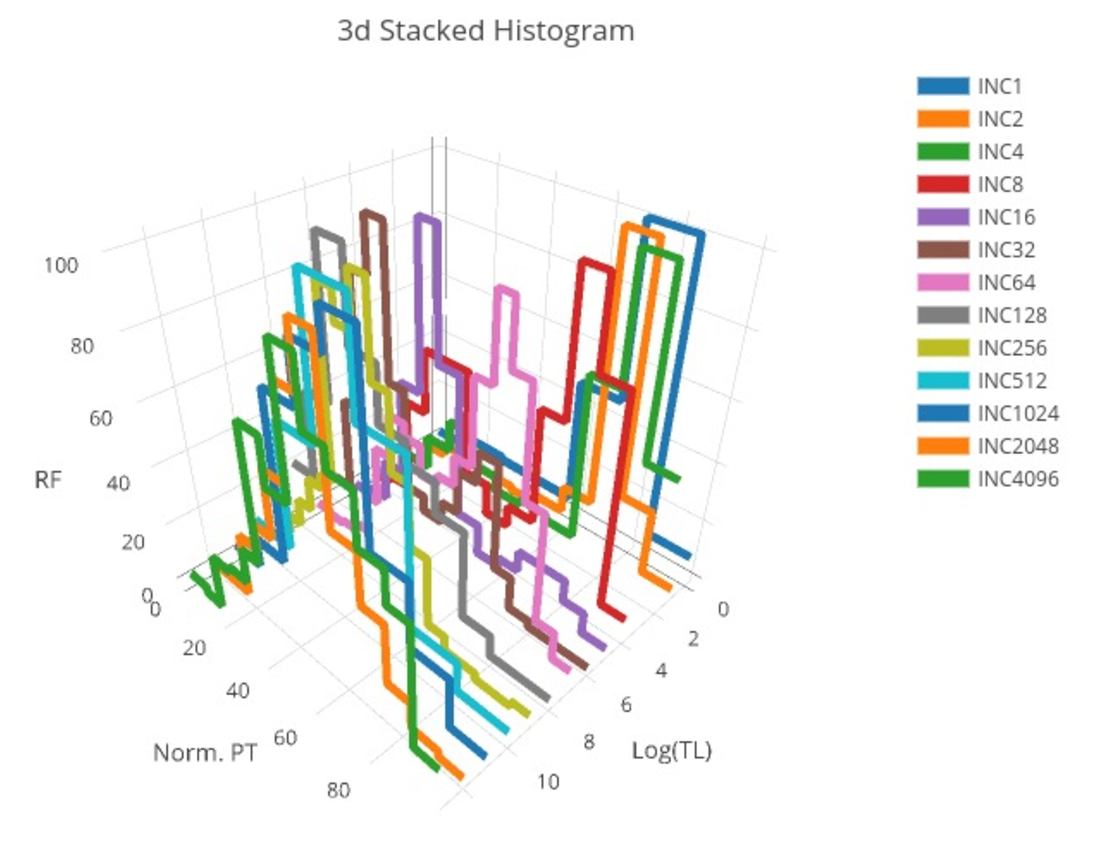
\includegraphics[scale=1]{u_s_time/3dplot_utime_only}\label{fig:3d_plot_u}
	\caption{3D histograms on INC: u time only~\label{fig:hist3d_u}}
\end{figure}

\clearpage
\pagebreak

\paragraph{Fitting the Histograms in Bi-normal Distributions:}
We ran Rob's code to obtain a bi-normal fit for each INC's run. 
Table~\ref{tab:binormal_fit} exhibits the two means (modes), standard deviations, and scales for each of the INC runs.

\begin{table}[h]
\begin{center}
\begin{tabular}{|l|l|l|l|l|l|l|} \hline
INC        & Mean 1 & Mean 2 & Std 1 & Std 2 & Scale 1 & Scale 2\\ \hline
INC1      & 1.66  & 4.73 & 1.03 & 0.54 & 0.104788 & 0.895212\\ \hline
INC2      & 2.33  & 7.07 & 2.38 & 0.54 & 0.159807 & 0.840193\\ \hline
INC4      & 2.17  & 7.89 & 0.99 & 0.86 & 0.209242 & 0.790758\\ \hline
INC8      & 3.51  & 9.15 & 1.10 & 1.08 & 0.388976 & 0.611024\\ \hline
INC16    & 4.04  & 9.53 & 0.98 & 1.28 & 0.828952 & 0.171048\\ \hline
INC32    & 2.76  & 8.26 & 1.28 & 1.12 & 0.725687 & 0.274313\\ \hline
INC64    & 6.36  & 12.02 & 1.64 & 1.62 &  0.347095 & 0.652905\\ \hline
INC128  & 4.21  & 8.64 & 1.82 & 3.40 & 0.410859 & 0.589141\\ \hline
INC256  & 6.08  & 14.61  & 3.59 & 3.75 & 0.124312 & 0.875688\\ \hline
INC512  & 1.60  & 12.43   & 11.51 & 4.47 & 0.075758 & 0.924242\\ \hline
INC1024 & 1.13  & 18.88  & 14.99 & 6.01 & 0.055255 & 0.944745\\ \hline
INC2048 & 29.93 & 52.92 & 8.53 & 6.59 & 1.001873 & -0.00187\\ \hline
INC4096 & 39.57 & 98.00 & 12.41 & 8.19 & 0.939756 & 0.060244\\ \hline
\end{tabular}
\end{center}
\vspace{-.2in}
\caption{Two means in mode computed for each INC~\label{tab:binormal_fit}}
\end{table}

\clearpage
\pagebreak

%\subsection{Absolute and Relative Variance over Increasing Task Lengths}
\paragraph{Absolute and Relative Variance over Increasing Task Lengths:}
Figure~\ref{fig:cv_inc} exhibits absolute and relative variances over increasing task lengths. 
More specifically, Figures~\ref{fig:overall_std} and~\ref{fig:overall_std_log} 
concern the PT standard deviations of all the runs including those two longest runs of INC8192 and INC16384 described in Table~\ref{tab:exp_notes2}. 
The x-axis is task length, and the y-axis standard deviation; Figure~\ref{fig:overall_std_log} is taken in log scale.
Figures~\ref{fig:overall_re} and~\ref{fig:overall_re2} shows 
the relative variance of the same data set---{\em coefficient of variation} (= standard deviation 
/ task length (or mean)). Both of the x and y axes in these two figures are taken in log scale. 
We also overlap a linear-square-fit of each case on the same figure. 

\begin{figure}[htp!]
	\centering
	\subfigure[Standard deviation (absolute)]{
		%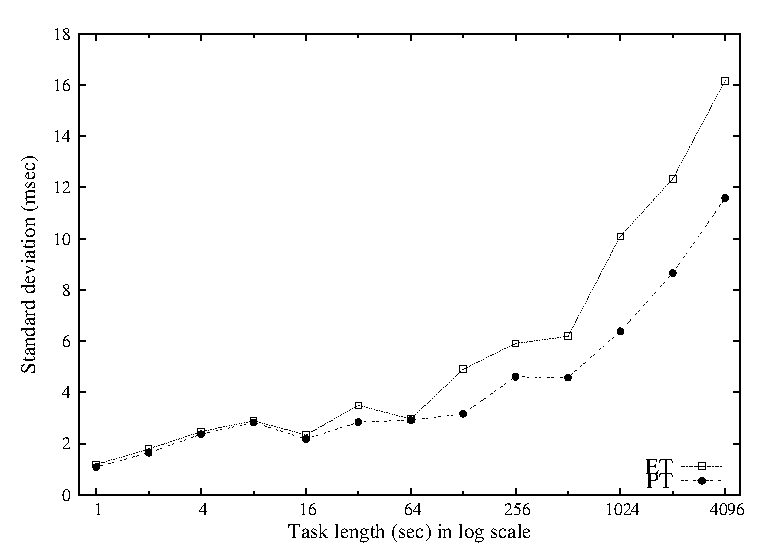
\includegraphics[scale=0.6]{u_s_time/overall_std.eps}
		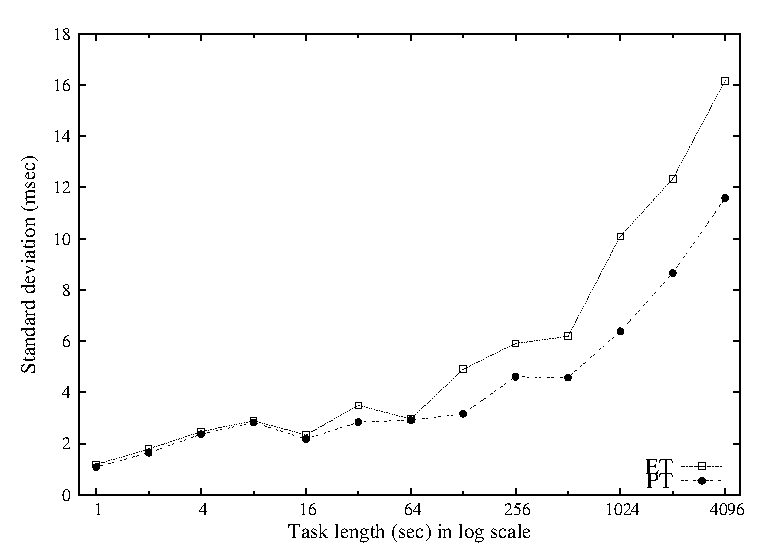
\includegraphics[scale=0.6]{u_s_time/new_overall_pt_std.eps}
		\label{fig:overall_std}
	}
	\subfigure[Standard deviation (absolute) in log scale]{
		%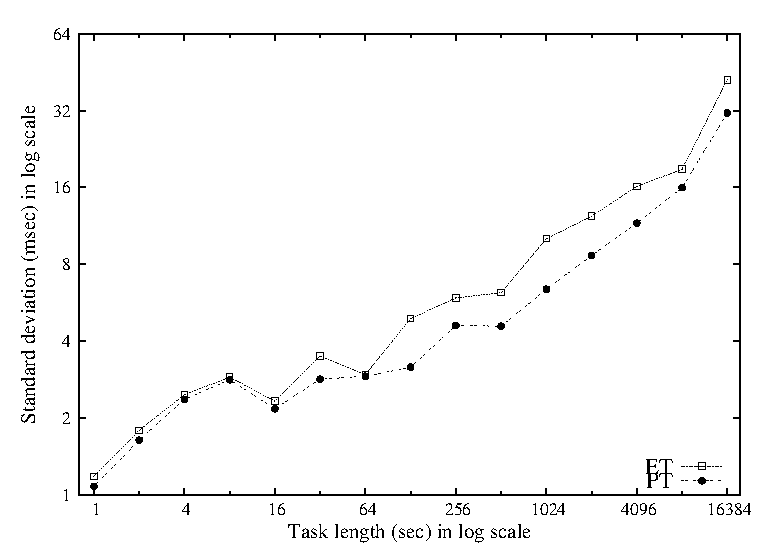
\includegraphics[scale=0.6]{u_s_time/overall_std_log.eps}
		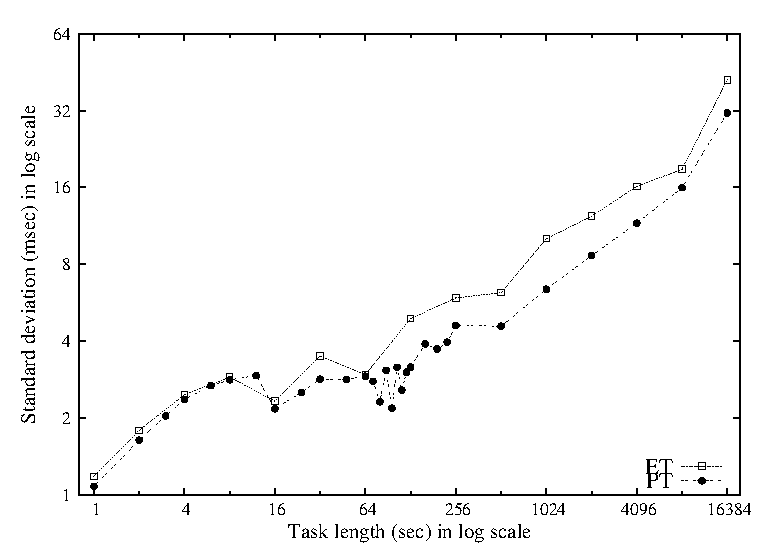
\includegraphics[scale=0.6]{u_s_time/new_overall_pt_std_log.eps}
		\label{fig:overall_std_log}
	}
	\subfigure[Coefficient of variation in log scale (relative): divisor=mean]{
		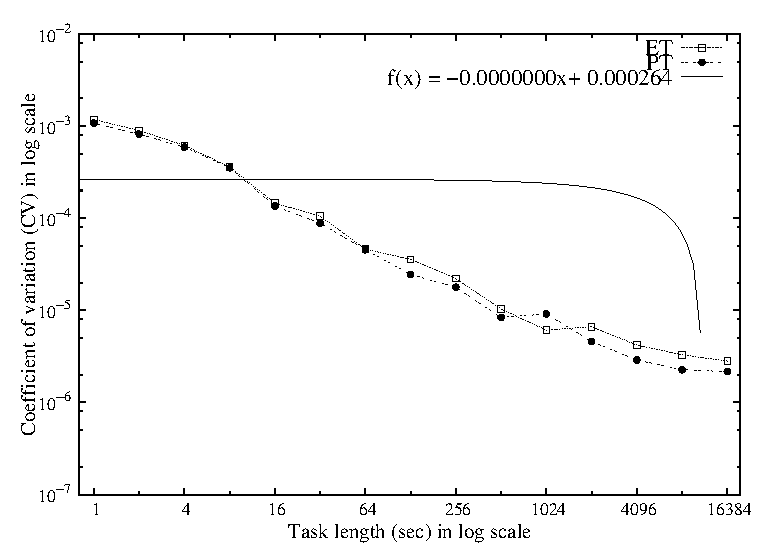
\includegraphics[scale=0.6]{u_s_time/overall_pt_re.eps}
		\label{fig:overall_re}
	}
	\subfigure[Coefficient of variation in log scale (relative): divisor=task length]{
		\includegraphics[scale=0.6]{u_s_time/new_overall_pt_re.eps}
		\label{fig:overall_re2}
	}
	\caption{Absolute and relative variances~\label{fig:cv_inc}}
\end{figure}

